% Document layout
\documentclass[a4paper,11pt]{article}
\usepackage[a4paper, inner=2.5cm , outer=2.5cm, top=2cm, bottom=2cm]{geometry}
\usepackage[usenames,dvipsnames]{color}
% Referencing & fonts
\usepackage[sort&compress]{natbib}
\setlength{\bibsep}{0.0pt}
\usepackage[font=small,labelfont=bf]{caption}
\usepackage[OT2,T1]{fontenc}
% Set formats for each heading level
\usepackage{sectsty}
\allsectionsfont{\usefont{OT1}{phv}{bc}{n}\selectfont}
\sectionfont{\color{MidnightBlue}} % sets colour of sections
\subsectionfont{\color{MidnightBlue}}  % sets colour of subsections
\subsubsectionfont{\color{MidnightBlue}}  % sets colour of subsections
% Other shit
\usepackage{algorithm}
\usepackage{amsfonts}
\usepackage{amsmath}
\usepackage{amssymb}
\usepackage{bbm}
\usepackage{booktabs}
\usepackage{epsfig}
\usepackage{float}
\usepackage[font=normalsize]{caption}
\usepackage{graphicx}
\usepackage{hyperref}
\usepackage{lineno}
\usepackage{mathtools}
\usepackage{sidecap}
\usepackage{sectsty}
\usepackage{verbatim}
\usepackage{wrapfig}
\usepackage{xcolor}
% Declarations
\DeclarePairedDelimiter\floor{\lfloor}{\rfloor}
\DeclareSymbolFont{cyrletters}{OT2}{wncyr}{m}{n}
\DeclareMathSymbol{\Sha}{\mathalpha}{cyrletters}{"58}
\DeclareMathSymbol{\sha}{\mathalpha}{cyrletters}{"57}
% Defined commands
 \newcommand{\prgname}[1]{\textcolor{NavyBlue}{\texttt{#1}}}
 \newcommand{\linkfont}[1]{\textcolor{BurntOrange}{\textbf{#1}}}
\newcommand{\shellcmd}[1]{\\\indent\indent\texttt{\$ #1}}
\newcommand{\shellctd}[1]{\\\indent\indent\texttt{#1}}
\newcommand{\ra}[1]{\renewcommand{\arraystretch}{#1}}
\begin{document}
\begin{figure}
\centering
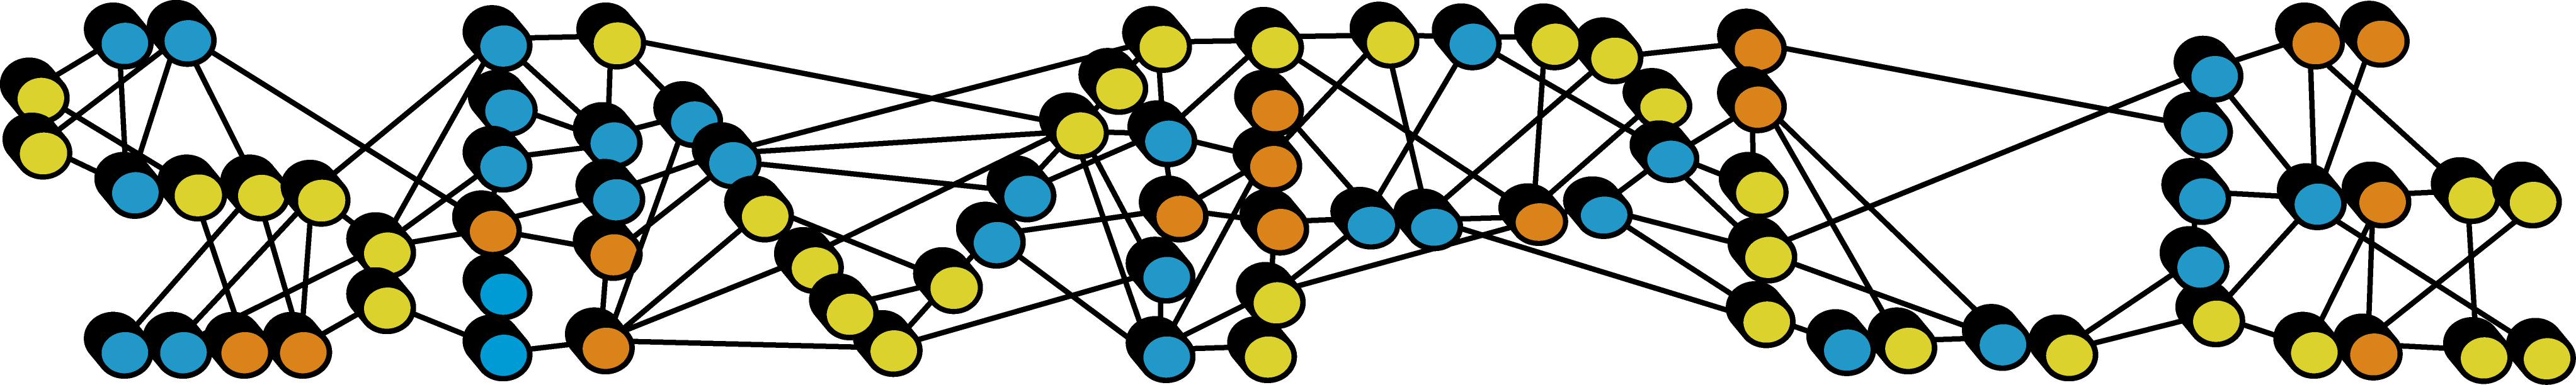
\includegraphics[keepaspectratio=true,scale=0.6]{./SIMPLE_logo/rawlogo}
%\caption{}
\end{figure}

\title{\prgname{The SIMPLE 2.5 Manual}}
\date{June 12, 2017}
\maketitle

\vspace{1em}
\begin{minipage}[ht]{0.48\textwidth}
\textbf{Contributors:}\\
cyril.reboul@monash.edu\\
michael.eager@monash.edu\\
dominika.elmlund@monash.edu\\
hans.elmlund@monash.edu\\
\textbf{Adress:}\\
Dept. Biochemistry and Molecular Biology\\
School of Biomedical Sciences\\
Monash University, Bldg. 77\\
Clayton, VIC, Australia, 3800\\
\textbf{Webpage:}\\
www.simplecryoem.com\\
\textbf{Contact:}\\
\url{http://simplecryoem.com/contact.html}\\
dominika@simplecryoem.com\\
\end{minipage}
\vspace{20pt}

\begin{quote}
\textbf{``Keep it SIMPLE stupid''}\\(\textit{Kelly Johnson}; lead engineer at the Lockheed Skunk Works, coined the famous KISS principle stating that systems work best if they are kept simple rather than made complex. Therefore, simplicity should be a key goal in design and unnecessary complexity should be avoided.)
\end{quote}

\begin{quote}
\textbf{``Everything should be made as SIMPLE as possible, but no SIMPLEr''}\\(\textit{Albert Einstein})
\end{quote}

\begin{quote}
\textbf{``Complex theories do not work, SIMPLE algorithms do''}\\(\textit{Vladimir N. Vapnik}; author of \textit{The Nature of Statistical Learning Theory})
\end{quote}
\clearpage

\tableofcontents{}
\clearpage

\section{About SIMPLE}

\textbf{S}ingle-particle \textbf{IM}age \textbf{P}rocessing \textbf{L}inux \textbf{E}ngine (\href{www.simplecryoem.com}{\textbf{\textcolor{BurntOrange}{SIMPLE}}}) is a program package for cryo-EM image processing, focusing on \textit{ab initio} 3D reconstruction of single-particles with any point-group symmetry. The SIMPLE back-end consists of an object-oriented numerical library written in modern Fortran. The SIMPLE front-end consists of a few standalone, interoperable components developed according to the ``Unix toolkit philosophy''.

SIMPLE is free software: you can redistribute it and/or modify it under the terms of the \href{http://www.gnu.org/copyleft/gpl.html}{\textbf{\textcolor{BurntOrange}{GNU General Public License}}} as published by the Free Software Foundation, either version 3 of the license, or (at your option) any later version. SIMPLE is distributed with the hope that it will be useful, but WITHOUT ANY WARRANTY; without even the implied warranty of MERCHANTABILITY or FITNESS FOR A PARTICULAR PURPOSE. See the \href{http://www.gnu.org/copyleft/gpl.html}{\textbf{\textcolor{BurntOrange}{GNU General Public License}}} for more details.

\subsection{What is new in SIMPLE release 2.5?}
\begin{itemize}
    \item[--] A new DDD movie pre-processing program \prgname{unblur} that implements motion correction based the same principal strategy as Grigorieff's program (hence the name). There are two important differences: automatic weighting of the frames using a correlation-based M-estimator and stochastic continuous optimisation of the shift parameters. This enables analysis of movies with severe pathologies due to radiation damage or extreme drift.
    \item[--] A new program \prgname{unblur\_tomo} for movie-processing of tomographic tilt-series.
    \item[--] Improved simultaneous 2D alignment and clustering with \prgname{prime2D} using a hybrid extremal/stochastic hill-climbing search approach, Wiener restoration-based CTF correction and acceleration of the search using Hadamard projection matching. It is now possible to generate sub-nanometer resolution \textit{ab initio} 3D reconstruction from class averages obtained with  \prgname{prime2D} in a about 10 minutes on a laptop (MacBook Pro mid 2015, 2.8 GHz Intel i7, four physical cores).
    \item[--] Improved \textit{ab initio} 3D reconstruction from class averages using stochastic neighbourhood hill-climbing for initialisation of the 3D orientation search, improving the success rate from around 40\% to 90-100\% for more challenging starting model generation problems, executed with program \prgname{ini3D\_from\_cavgs}
    \item[--] Serial CPU code optimisation through data re-organisation and pipelining.
    \item[--] Improved parallel CPU performance through load balancing as well as data and algorithm re-organisation. It is now possible to process data sets of realistic size on laptops or lightweight workstations that cost less than 2,000 USD.
    \item[--] High-level workflows for 2D analysis and initial 3D model production that automates initialisation, update of search parameters and dynamic down-scaling of the images for improved performance.
\end{itemize}

\section{File Formats}

\subsection{Image File Formats}
SIMPLE supports SPIDER (\texttt{*.spi}) and MRC (\texttt{*.mrc}) formats for image stacks and volumes. The MRC file handling classes are shared with the the FREALIX program for helical reconstruction \citep{Rohou:2014aa}. RELION \citep{Scheres:2012aa} uses the convention that MRC stacks have the suffix \texttt{*.mrcs} and volumes the suffix \texttt{*.mrc}. This is to overcome the annoyance that it is not possible to tell from an MRC file header whether a MRC file is a volume or a stack. With SIMPLE you can select to use either the \texttt{*.mrcs} or \texttt{*.mrc} suffix for stacks. The way that we keep track of whether a file is a volume or stack is via the command line key value. The key-value pairs \texttt{vol1=rec.mrc} and \texttt{vol2=rec2.mrc} refer to volumes whereas the key-value pairs \texttt{stk=ptcls.mrc} and \texttt{stk2=ptcls2.mrc} refer to stacks.

\subsection{SIMPLE Parameter File Format}
The SIMPLE text-files used for parameter input/output use a \texttt{key=value} syntax of the form
\begin{verbatim}
e1=80. e2=100. e3=5.5 x=1.23 y=4.25 dfx=2.56 dfy=2.54 angast=30.5 state=1
\end{verbatim}
to represent per-particle information. Internally, the orientation information is stored in a dynamic hash data structure, which gives the file format high flexibility. Therefore, writing conversion scripts to allow interchange of parameters between SIMPLE and other packages is easy. SIMPLE uses the same conventions as FREALIGN \citep{Grigorieff:2007aa} to represent orientations and CTF parameters. The CTF parameterisation obtained by CTFFIND \citep{Mindell:2003aa} can be directly plugged into SIMPLE, for example by creating a file \texttt{deftab.txt}, looking like
\begin{verbatim}
kv=300 cs=2.7 fraca=0.07 dfx=2.56 dfy=2.76 angast=30.5
kv=300 cs=2.7 fraca=0.07 dfx=3.50 dfy=3.33 angast=60.0
kv=300 cs=2.7 fraca=0.07 dfx=1.98 dfy=2.02 angast=120.5
...
\end{verbatim}
and adding \texttt{deftab=deftab.txt} and \texttt{ctf=yes} to the PRIME command line (if the images are phase-flipped, this should be indicated by \texttt{ctf=flip}). Note that we now include \texttt{kv}, \texttt{cs}, and \texttt{fraca} in the document listing the CTF parameters. Having all the CTF parameters listed per particle allows easy merging of data sets from different microscopes. SIMPLE now implements a wrapper program for CTFFIND version 4.1.X and newer, producing a SIMPLE conforming document by executing CTFFIND in parallel (via \texttt{simple\_distr\_exec prg=ctffind}). If you have obtained CTF parameters with CTFFIND by other means (via RELION, for example) you can provide a plain text file with the two defocus values and the angle of astigmatism to the SIMPLE program \prgname{makedeftab} and it will take care of the formatting and unit conversions for you.

\subsection{Parameter File Conversions}
The \texttt{SIMPLE/scripts} folder contains a perl-script (\texttt{convert\_frealign2simple.pl}) to convert a Frealing parameter file to a SIMPLE parameter file. This is easy, since both software internally use the \href{http://spider.wadsworth.org/spider_doc/spider/docs/euler.html}{\textbf{\textcolor{BurntOrange}{Spider Euler angle convention}}}. Other packages may use other conventions. There's also a \texttt{convert\_relion2simple.pl} for extracting CTF parameters from RELION \texttt{*.star} files and a \texttt{relion2emanbox.pl} script for converting box files obtained with RELION to the EMAN \texttt{*.box} format used by SIMPLE.

\section{Installation}
\label{install}

\subsection{System requirements}
\label{sysreq}

\subsubsection{Hardware}
\label{hardware}

\begin{itemize}
	\item [CPU]
	\begin{itemize}
		\item[--] Linux
		\item[--] MacOSX (Yosemite and El Capitan, \textit{i.e.} 10.10 and above)
	\end{itemize}
\end{itemize}

\subsubsection{Software}
\label{soft}

\begin{itemize}
	\item [CPU]
	\begin{itemize}
		\item[--] GNU tool chain 4.9 and above.
		\item[--] FFTW-3 (The Fastest Fourier Transform in the West library)
	\end{itemize}
\end{itemize}

\subsection{Compiling SIMPLE}
\label{compilepc}
To check the compiler version, execute
\begin{verbatim}
@!#> gfortran --version
GNU Fortran (GCC) 4.9.1
Copyright (C) 2014 Free Software Foundation, Inc.
\end{verbatim}
To check whether the FFTW library is installed, open the package manager installed on our system (in our case \texttt{Synaptic} but other systems may have others, such as \texttt{YaST}, \texttt{apt} etc.) and search for \texttt{fftw} and see that the \texttt{libfftw3-single-3} is installed on the system. We \texttt{cd} to the directory  where we have our software installed (\texttt{<my software location>}) and copy the tar ball there
\begin{verbatim}
@!#> cd <my software location>
@!#> cp ~/Downloads/simple.tar.gz .
\end{verbatim}
Next, we unpack the tar ball and \texttt{cd} to the simple directory
\begin{verbatim}
@!#> gunzip simple.tar.gz
@!#> tar -xvf simple.tar
@!#> cd simple/
\end{verbatim}
We open the \texttt{simple\_user\_input.pm} file in our favourite text editor. There are a few lines that needs to be edited:
\begin{verbatim}
...
26  # enter the SIMPLE root path
27  our$SIMPLE_PATH="/Users/hael/src/fortran/simple";
...
\end{verbatim}
Line 27 \texttt{our\$SIMPLE\_PATH = "/Users/hael/src/fortran/simple/"} is replaced with\\
\texttt{our\$SIMPLE\_PATH$=$"<my software location>/simple/"}. This is the path in which the software will be installed.
\begin{verbatim}
...
46  our$FCOMPILER = "gfortran-5";
...
\end{verbatim}
Line 46 \texttt{our\$FCOMPILER = "gfortran-5";} is the command that executes the \texttt{gfortran} compiler. On a mac, using the fink package manager, this command would be \texttt{/sw/bin/gfortran}.
\begin{verbatim}
...
49  # enter the fftw lib default: /usr/lib/x86_64-linux-gnu for [linux]
50  #                             /usr/local/lib for [MacOSX]
51  our$FFTW_LIB="/usr/lib/x86_64-linux-gnu";
52  # on clusters we need extra path after module load fftw/3.3.4-gcc
53  our$FFTW_INC="/usr/include/";
...
\end{verbatim}
Lines 51 and 53 specify the FFTW library and include directories. On a mac, using the fink package manager, these locations would be \texttt{our\$FFTW\_LIB="/sw/lib";} and \texttt{our\$FFTW\_INC="/sw/include/";}, respectively. We save and close the configuration file and execute:
\begin{verbatim}
@!#> ./compileSIMPLE.pl 
*********************************************************
* Checking and printing the input directories...        *
*********************************************************
SIMPLE_PATH          : /Users/hael/src/fortran/simple
SIMPLE_SRC_PATH      : /Users/hael/src/fortran/simple/src/simple_main
SIMPLE_PROD_PATH     : /Users/hael/src/fortran/simple/production
SIMPLE_TEST_PROD_PATH: /Users/hael/src/fortran/simple/production/simple_tests
SIMPLE_SCRIPTS_PATH  : /Users/hael/src/fortran/simple/scripts
*********************************************************
Moving to dir: /Users/hael/src/fortran/simple/src/simple_main
Executing simple_args_generator.pl in dir: /Users/hael/src/fortran/simple...
Moving to dir: /Users/hael/src/fortran/simple
Generating Makefile_macros: /Users/hael/src/fortran/simple
/sw/bin/gfortran -c -fimplicit-none -fall-intrinsics -ffree-form -cpp -fpic...
...
darwin, Platform = 0
Architecture: darwin-thread-multi-2level

Moving to dir: /Users/hael/src/fortran/simple/production
Generating compile_and_link: /Users/hael/src/fortran/simple/production
Moving to dir: /Users/hael/src/fortran/simple
Compiling production codes:
>>> COMPILING & LINKING: simple_test_shelliter
>>> COMPILING & LINKING: simple_test_autoscale
>>> COMPILING & LINKING: simple_test_scatsrch
>>> COMPILING & LINKING: simple_test_ft_expanded
>>> COMPILING & LINKING: simple_exec
>>> COMPILING & LINKING: simple_test_volpft_srch
>>> COMPILING & LINKING: simple_test_srch
>>> COMPILING & LINKING: simple_test_units
>>> COMPILING & LINKING: simple_test_cartcorr_sanity
>>> COMPILING & LINKING: simple_test_imgfile
>>> COMPILING & LINKING: simple_distr_exec
Compilation of SIMPLE completed in dir: /Users/hael/src/fortran/simple
\end{verbatim}
Compilation was succesful and we see that a new directory \texttt{/bin} has been created in the simple directory in addition to two text files \texttt{add2.bashrc} and \texttt{add2.tcshrc}
\begin{verbatim}
@!#> cat add2.bashrc 
export SIMPLE_EMAIL="my.name@uni.edu"
export SIMPLE_QSYS="local"
export SIMPLE_PATH=/Users/hael/src/fortran/simple
export PATH=${SIMPLE_PATH}/scripts:${SIMPLE_PATH}/bin:$PATH
@!#> cat add2.tcshrc 
setenv SIMPLE_EMAIL="my.name@uni.edu"
setenv SIMPLE_QSYS="local"
setenv SIMPLE_PATH /Users/hael/src/fortran/simple
set path=(${SIMPLE_PATH}/scripts ${SIMPLE_PATH}/bin $path)
\end{verbatim}
On this machine we use the bash shell, so we add the lines in \texttt{add2.bashrc} to the \texttt{.bashrc} file. This is done by using a text editor, such as \texttt{gedit}, to edit the hidden file \texttt{.bashrc} located in your home folder.
\begin{verbatim}
@!#> cd
@!#> gedit .bashrc 
\end{verbatim}

\subsection{Compilation troubleshooting}
\label{compiletrouble}

\subsubsection{FFTW}
If not already installed, the FFTW-3 library needs to be installed. Most Linux package managers \texttt{YaST}, \texttt{Synaptic}, \texttt{apt-get} etc. provide the FFTW-3 library. On a Mac system the \texttt{Fink} and \texttt{Macports} package managers provide the FFTW-3 library or it can be obtained from: \url{http://www.fftw.org/install/mac.html}. SIMPLE relies on the single-precision FFTW library. Typically we will need to
\begin{verbatim}
@!#> ./configure --enable-floats --enable-threads
@!#> make
@!#> sudo make install
\end{verbatim}
The \texttt{--enable floats} \texttt{--enable-threads} directives are critical as SIMPLE uses multi-threaded single-precision Fourier transforms. We check that we have in the lib folder (typically: \texttt{/usr/local/lib/}):
\begin{verbatim}
libfftw3.a libfftw3.la
libfftw3f.a libfftw3f.la
libfftw3f_threads.a libfftw3f_threads.la
\end{verbatim}

\subsection{Installation on a Linux Cluster}
\label{inst_clusters_linux}

Installation on a Linux cluster is essentially the same as on a Linux workstation with the exception that the appropriate modules need to be loaded before installation and execution. On a typical SLURM cluster
\begin{verbatim}
@!#> module load fftw/3.3.4-gcc
@!#> module load gcc/4.9.1
@!#> module load lapack/3.4.2 
\end{verbatim}
The instructions for how to execute SIMPLE in distributed environments (clusters or workstations with more than one CPU socket) are described below \label{distr}.

\subsection{Testing the SIMPLE Installation}
To ensure that SIMPLE has been correctly installed, we recommend running the application \prgname{simple\_test\_install}. It will test the most important components in the SIMPLE library  (those used by \prgname{prime2D} and \prgname{prime3D}). Execute
\begin{verbatim}
@!#> simple_test_install 
\end{verbatim}
The program will create its own folder (\texttt{SIMPLE\_TEST\_INSTALL*date*}) where temporary files and information about each test are stored. Upon succesful completion you should see
\begin{verbatim}
**** SIMPLE_TEST_INSTALL NORMAL STOP ****
\end{verbatim}
\prgname{simple\_test\_install} can be executed anywhere. After execution, the folder created can be safely removed. If any of the individual tests fail an error message will be displayed. If you detect an error, please carefully check the SIMPLE and FFTW installations and the \texttt{gfortran} version. If you still have issues, please file a help ticket on the webpage.

\section{SIMPLE Usage}

\subsection{SIMPLE Help Tools}
In attempt to reduce the dependency on the manual, we have packaged a lot of the documentation in the software itself. For example
\begin{verbatim}
@!#> simple_exec prg=list
automask2D
automask3D
binarise
boxconvs
cavgassemble
cenvol
check2D_conv
check3D_conv
...
\end{verbatim}
lists all programs executed with \texttt{simple\_exec} (shared-memory parallelisation) and
\begin{verbatim}
@!#> simple_distr_exec prg=list
comlin_smat
ctffind
ini3D_from_cavgs
makecavgs
prime2D
prime3D
prime3D_init
recvol
symsrch
tseries_track
unblur
unblur_ctffind
unblur_tomo
\end{verbatim}
lists all distributed workflows executed with \texttt{simple\_distr\_exec}. If you don't quite remember which program you are looking for but remember that it was called \texttt{prime} something, you could execute
\begin{verbatim}
@!#> simple_distr_exec prg=list | grep prime
prime2D
prime3D
prime3D_init
\end{verbatim}
If you want a description for a particular program, for example \prgname{prime2D}, execute
\begin{verbatim}
@!#> simple_distr_exec prg=prime2D describe=yes
is a reference-free 2D alignment/clustering algorithm adopted from the 
prime3D probabilistic ab initio 3D reconstruction algorithm
\end{verbatim}
To obtain a description of the what command line options are available, execute
\begin{verbatim}
@!#> simple_distr_exec prg=prime2D
USAGE:
bash-3.2$ simple_exec prg=simple_program key1=val1 key2=val2 ...

REQUIRED
stk  = particle stack with all images(ptcls.ext)
smpd = sampling distance, same as EMANs apix(in A)
msk  = mask radius(in pixels)
ncls = # clusters
ctf  = ctf flag(yes|no|flip)

OPTIONAL
nparts    = # partitions in distributed exection
chunksz   = # images/orientations in chunk
nthr      = # OpenMP threads{1}
ncunits   = # computing units, can be < nparts{nparts}
deftab    = text file with CTF info(*.txt/*.asc)
refs      = initial2Dreferences.ext
oritab    = table (text file) of orientations(*.asc/*.txt)
hp        = high-pass limit(in A)
lp        = low-pass limit(in A)
lpstart   = start low-pass limit(in A){15}
lpstop    = stop low-pass limit(in A){8}
cenlp     = low-pass limit for binarisation in centering(in A){30 A}
trs       = maximum halfwidth shift(in pixels)
automsk   = envelope masking(yes|no|cavg){no}
amsklp    = low-pass limit for envelope mask generation(in A)
inner     = inner mask radius(in pixels)
width     = falloff of inner mask(in pixels){10}
startit   = start iterating from here
maxits    = maximum # iterations
filwidth  = width of filament (in A)
center    = center image(s)/class average(s)/volume(s)(yes|no){no}
autoscale = automatic down-scaling(yes|no){yes}
oritab3D  = table (text file) of 3D orientations(*.asc/*.txt)
\end{verbatim}

\subsection{Execution of SIMPLE}
SIMPLE is executed primarily via \texttt{simple\_distr\_exec} that implements higher level workflows intended for distributed execution on workstations and clusters using a hybrid parallelisation model (distributed \textit{and} shared memory). SIMPLE can also be executed via \texttt{simple\_exec}, which implements all individual SIMPLE programs and runs in shared-memory parallelisation mode. Please, beware that the high-level workflows (\prgname{prime2D} and \prgname{ini3D\_from\_cavgs}, for example) can \textit{only} be executed via the distributed execution route. In cluster environments using a job scheduler (PBS, SLURM and SGE are supported by SIMPLE) the file \texttt{simple\_distr\_config.env} in the current working directory controls the execution.
\begin{verbatim}
bash-3.2$ cat simple_distr_config.env 
# CONFIGURATION FILE FOR DISTRIBUTED SIMPLE EXECUTION

# ABSOLUTE PATH TO SIMPLE ROOT DIRECTORY
simple_path           = /scratch/m3earlyadopters/simple/simple/

# ESTIMATED TIME PER IMAGE (IN SECONDS)
time_per_image        = 600

# USER DETAILS
user_account          = el85 
user_email            = hans.elmlund@monash.edu
user_project          = 

# QSYS DETAILS (qsys_name=<local|slurm|pbs>)
qsys_name             = slurm
qsys_partition        = m3a
qsys_qos              =
qsys_reservation      = simple

# JOB DETAILS
job_ntasks            = 1
job_memory_per_task   = 48000
job_name              = taf-dna-part2
job_ntasks_per_socket = 1
\end{verbatim}
This file is auto-generated on workstations, but it needs to be edited by the user in cluster environments. If you need help configuring distributed SIMPLE execution, please file a help ticket on the webpage. The two most important parameters for distributed execution is the number of partitions \texttt{nparts} and the number of shared-memory CPU threads \texttt{nthr}. A rule of thumb for good performance on multi-socket workstations is to minimise the number of parts and maximising the number of threads subject to never having fewer parts than sockets. The shared memory parallelisation does not benefit from the use of a larger number of threads than the number of logical threads available on a socket. To check the number of processors on a linux system, execute \texttt{nproc} in the terminal. Consider a heterogeneous cluster with N nodes, two CPU sockets per node and six CPUs per socket.
\begin{SCfigure}[][h]
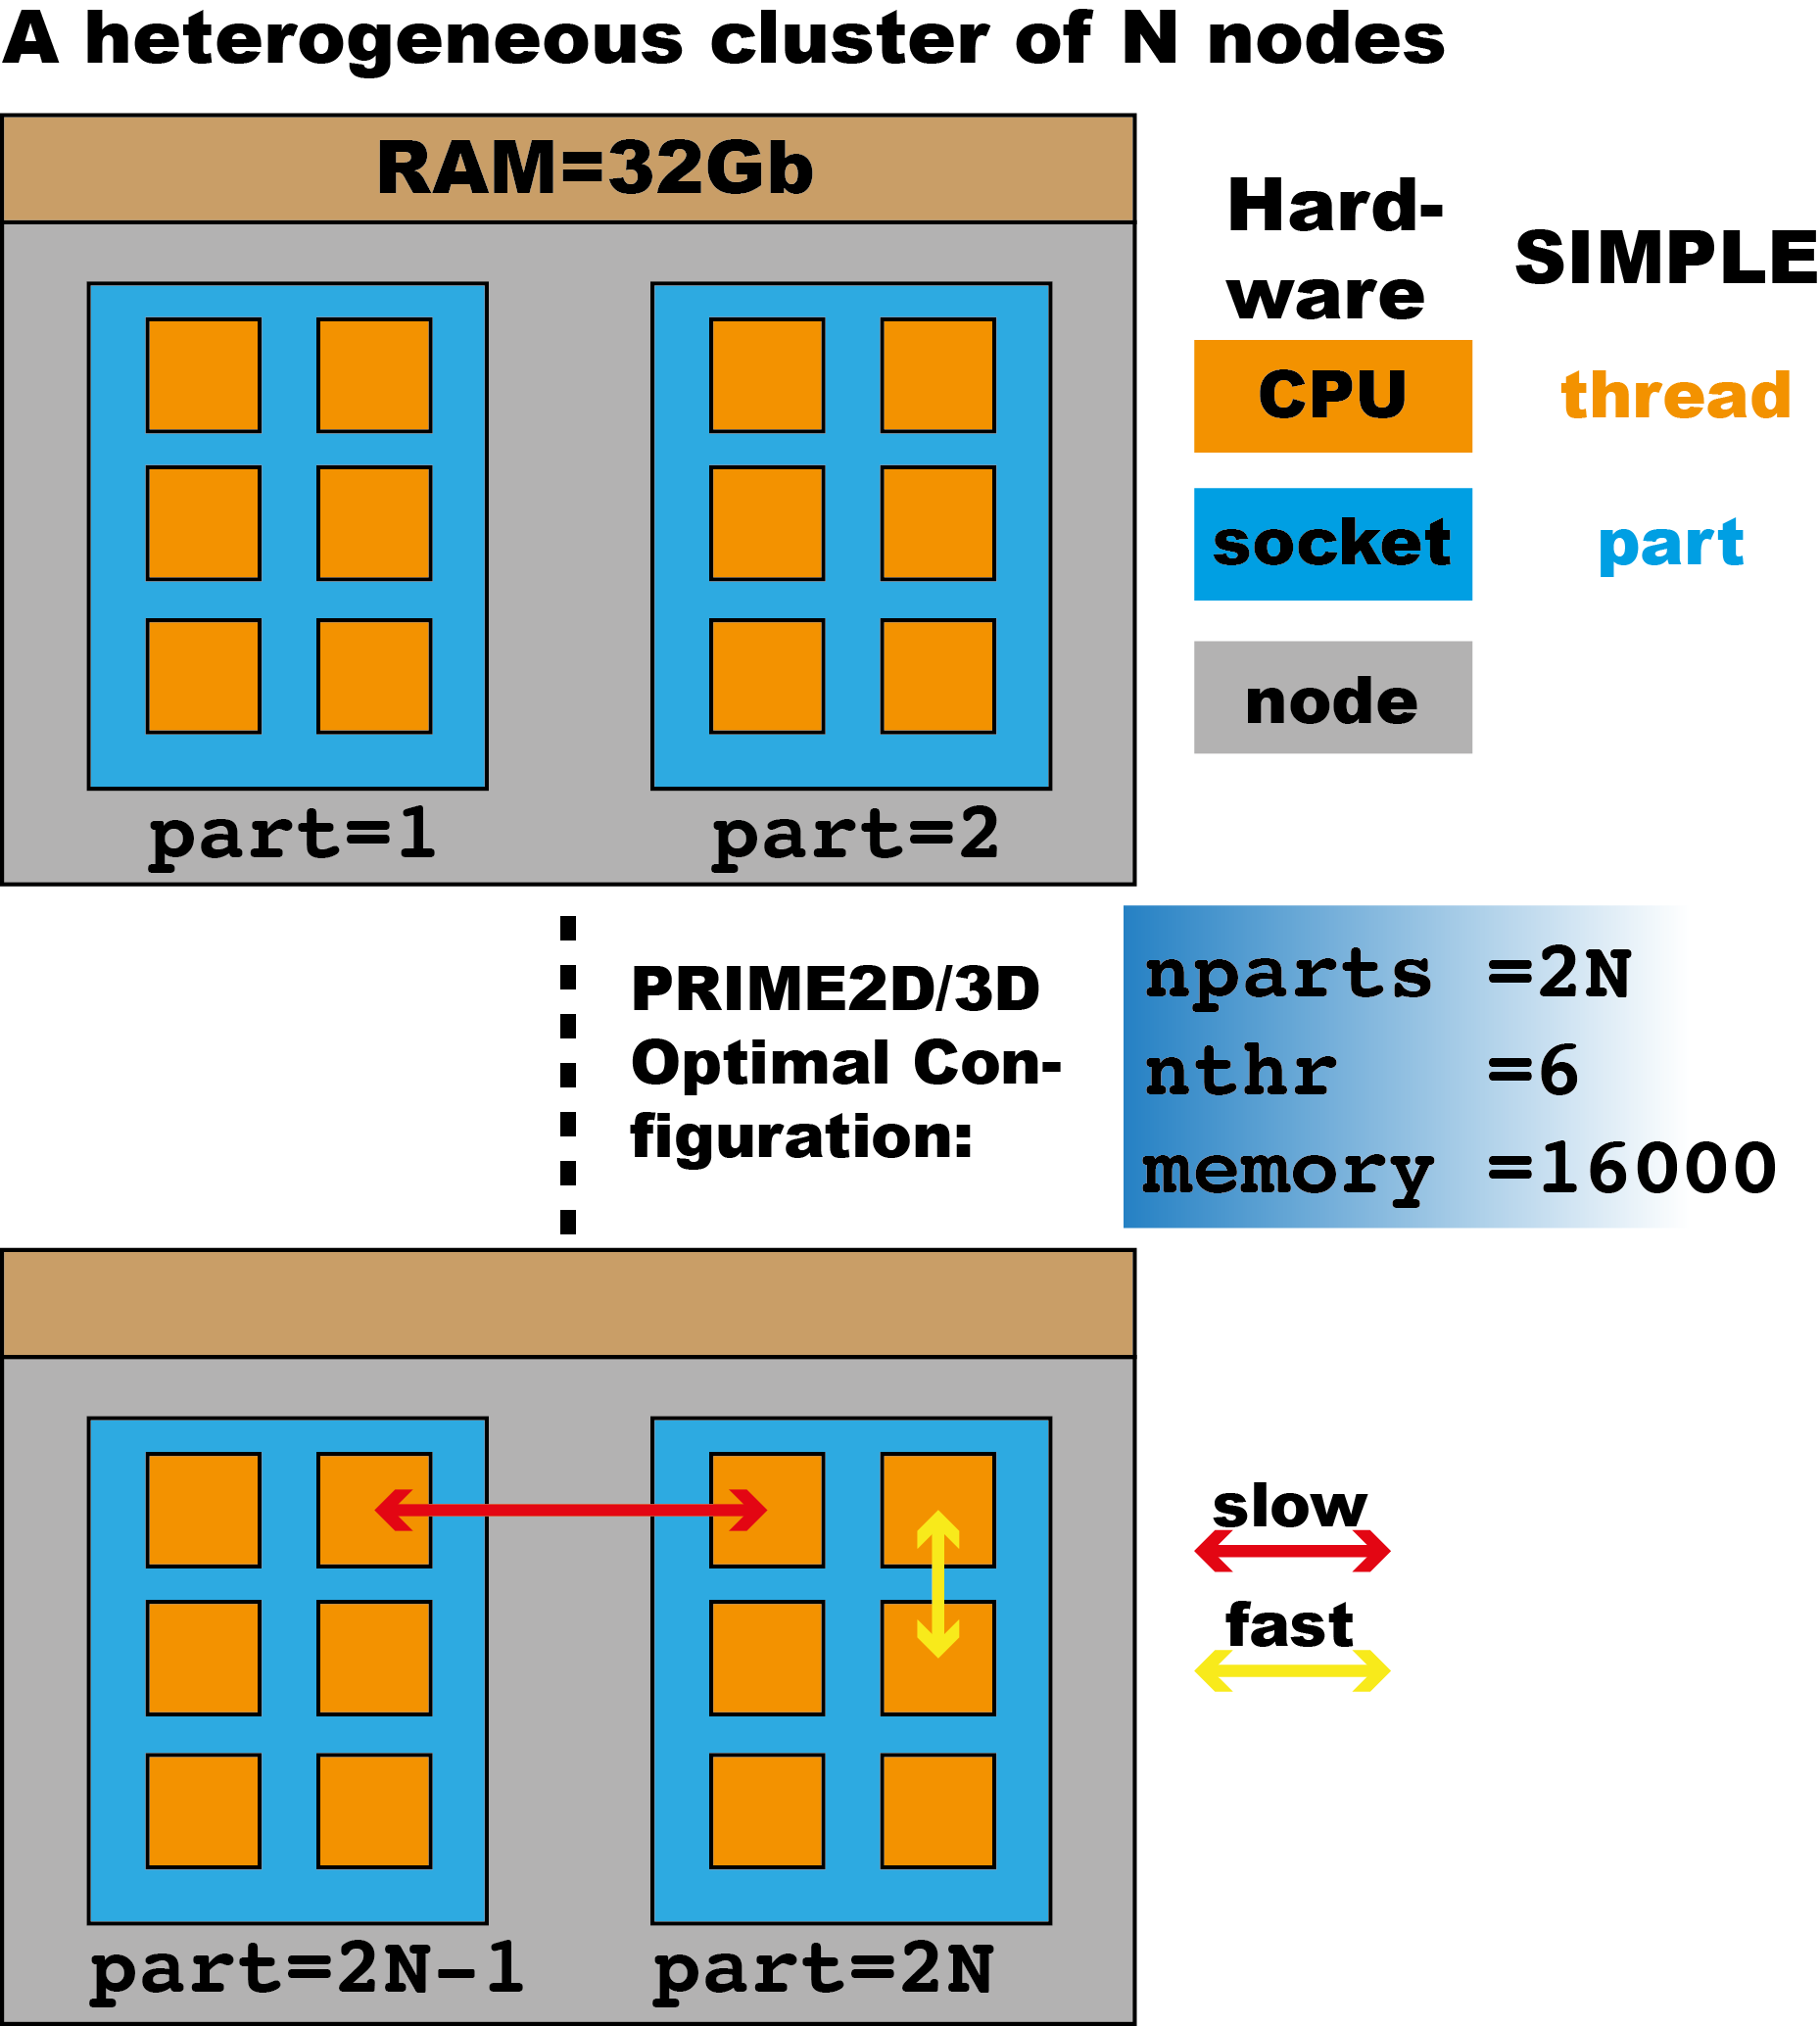
\includegraphics[keepaspectratio=true,scale=0.6]{./CPUtopo/cputopo}
\caption{\textbf{Configuration of the parallel PRIME-2D/3D execution on a heterogeneous cluster.} We here represent the nodes in  a heterogeneous cluster by two sockets with six CPUs each and 32Gb RAM/node. The best performance of PRIME--2D/3D is going to be obtained by partitioning  the jobs into \texttt{npart=2N} partitions, where \texttt{N} is the number of nodes. Each partition will then execute six threads \texttt{nthr=6} and these six threads will get access to half the RAM on the node (\texttt{memory=16000}) because we have two sockets per node that need to share the RAM between them}
\end{SCfigure}
If you are unsure how to configure your SIMPLE execution please file a help ticket.

We normally let \prgname{simple\_distr\_exec} run in the background on the login node of our cluster. An example of how to distribute \prgname{prime2D} using ten nodes is provided below.
\begin{verbatim}
@!#> nohup simple_distr_exec prg=prime2D stk=ptcls.mrc smpd=1.77 msk=100
ncls=600 nthr=8 nparts=10 >> PRIME2DOUT &
\end{verbatim}
Another option available on clusters that use the SLURM scheduler is to use the \texttt{srun} command for \prgname{simple\_distr\_exec} via
\begin{verbatim}
@!#> srun --ntasks=1 --ntasks-per-socket=1 --cpus-per-task=1 --mem=32000 
--time=2-0:0:0 --output=PRIME2DOUT.%j --error=PRIME2DERR.%j
simple_distr_exec prg=prime2D stk=ptcls.mrc smpd=1.77 msk=100
ncls=600 nthr=8 nparts=10 &
\end{verbatim}
However, beta testers have reported that srun job sometimes dies with no warning, possibly because of the low tolerance for network errors. A more robust route may be to use \texttt{sbatch} as follows
\begin{verbatim}
@!#>  sbatch -p MYCLUSTER --wrap="simple_distr_exec prg=prime2D stk=ptcls.mrc 
smpd=1.77 msk=100 ncls=600 nthr=8 nparts=10 >> PRIME2DOUT"
\end{verbatim}
where the \texttt{--wrap} flag automatically generates a bash script for the given command.

\subsection{From Movies to \textit{ab initio} 3D reconstruction}
These steps describe a typical SIMPLE workflow.
\begin{enumerate}
\item DDD (Direct Detector Device) movie alignment and frame-weighting using SIMPLE program \prgname{unblur}, executed with \texttt{simple\_distr\_exec}
\item CTF parameter identification with the SIMPLE program \prgname{ctffind}, wrapping CTFFIND4 \citep{rohou2015ctffind4}, executed with \texttt{simple\_distr\_exec}
\item Particle identification using EMAN2 \citep{Tang:2007aa} to generate \texttt{*.box} files
\item Particle extraction with SIMPLE program \prgname{extract}, executed with \texttt{simple\_exec}
\item 2D analysis using the SIMPLE \prgname{prime2D} distributed workflow, executed with \texttt{simple\_distr\_exec}
\item \textit{Ab initio} 3D reconstruction from class averages using the SIMPLE \prgname{ini3D\_from\_cavgs} distributed workflow, executed with \texttt{simple\_distr\_exec}
\item Mapping of class average selection and 3D class orientations to the particles using SIMPLE program \prgname{map2ptcls}, executed with \texttt{simple\_exec}
\item Reconstruction of a 3D map from the individual particle images with SIMPLE program \prgname{recvol}, executed with \texttt{simple\_distr\_exec}
\item Map refinement will be part of release 3.0
\end{enumerate}
For descriptions for how to execute the individual steps, please refer to the documentation of each program (below).

\section{Command Line Dictionary}
\begin{tabular}{ll}
\texttt{acf             }&{ calculate autocorrelation function(yes|no)\{no\}}\\
\texttt{amsklp          }&{ low-pass limit for envelope mask generation(in \AA{})}\\
\texttt{angastunit      }&{ angle of astigmatism unit (radians|degrees)\{degrees\}}\\
\texttt{angerr          }&{ angular error(in degrees)\{0\}}\\
\texttt{append          }&{ append in context of files(yes|no)\{no\}}\\
\texttt{astigerr        }&{ astigmatism error(in microns)}\\
\texttt{astigstep       }&{ step size for astigamtism search(in microns)}\\
\texttt{async           }&{ asynchronous mode of operation(yes|no)\{no\}}\\
\texttt{athres          }&{ angular threshold(in degrees)}\\
\texttt{automsk         }&{ envelope masking(yes|no|cavg)\{no\}}\\
\texttt{autoscale       }&{ automatic down-scaling(yes|no)\{yes\}}\\
\texttt{avg             }&{ calculate average(yes|no)}\\
\texttt{bfac            }&{ bfactor for sharpening/low-pass filtering(in \AA{}**2)\{200.\}}\\
\texttt{bfacerr         }&{ bfactor error in simulated images(in \AA{}**2)\{0\}}\\
\texttt{bin             }&{ binarise image(yes|no)\{no\}}\\
\texttt{binwidth        }&{ binary layers grown for molecular envelope(in pixels)\{1\}}\\
\texttt{box             }&{ square image size(in pixels)}\\
\texttt{boxconvsz       }&{ size of box used for box-convolution(in pixels)}\\
\texttt{boxfile         }&{ file with EMAN particle coordinates(*.txt/*.asc)}\\
\texttt{boxtab          }&{ table (text file) of files with EMAN particle coordinates(*.txt/*.asc)}\\
\texttt{cenlp           }&{ low-pass limit for binarisation in centering(in \AA{})\{30 A\}}\\
\texttt{center          }&{ center image(s)/class average(s)/volume(s)(yes|no)\{no\}}\\
\texttt{chunksz         }&{ \# images/orientations in chunk}\\
\texttt{class           }&{ cluster identity}\\
\texttt{clip            }&{ clipped image box size(in pixels)}\\
\texttt{clustvalid      }&{ validate clustering(yes|homo|no)\{no\}}\\
\texttt{comlindoc       }&{ shc\_clustering\_nclsX.txt}\\
\texttt{compare         }&{ do comparison(yes|no)\{no\}}\\
\texttt{corner          }&{ corner size(in pixels)\{0\}}\\
\texttt{countvox        }&{ count \# voxels(yes|no)\{no\}}\\
\texttt{cs              }&{ spherical aberration constant(in mm)\{2.7\}}\\
\texttt{ctf             }&{ ctf flag(yes|no|flip)}\\
\texttt{ctffind\_doc     }&{ per-micrograph CTF parameters to transfer}\\
\texttt{ctfsq           }&{ apply ctf**2 to the images(yes|no)\{no\}}\\
\texttt{ctfsqspec       }&{ filename of ctf**2 spectrum\{ctfsqspec\_state01.bin\}}\\
\texttt{ctfstats        }&{ calculate ctf statistics(yes|no)\{no\}}\\
\texttt{cube            }&{ side size(in pixels)\{0\}}\\
\texttt{dcrit\_rel       }&{ critical distance relative to box(0-1)\{0.5\}}\\
\texttt{defocus         }&{ defocus(in microns)\{3.\}}\\
\texttt{deftab          }&{ text file with CTF info(*.txt/*.asc)}\\
\texttt{dferr           }&{ defocus error(in microns)\{1.0\}}\\
\texttt{dfmax           }&{ maximum expected defocus(in microns)}\\
\texttt{dfmin           }&{ minimum expected defocus(in microns)}\\
\texttt{dfunit          }&{ defocus unit (A|microns)\{microns\}}\\
\texttt{dir             }&{ directory}\\
\texttt{dir\_movies      }&{ grab *.mrc/*.mrcs files from here}\\
\texttt{dir\_reject      }&{ move rejected files to here\{rejected\}}\\
\texttt{dir\_select      }&{ move selected files to here\{selected\}}\\
\texttt{dir\_target      }&{ put output here}\\
\texttt{discrete        }&{ discrete(yes|no)\{no\}}\\
\texttt{diverse         }&{ diverse or not flag (yes|no)\{no\}}\\
\texttt{doclist         }&{ list of oritabs for different states}\\
\texttt{dopick          }&{ execute picking step (in preproc)\{yes\}}\\
\end{tabular}

\begin{tabular}{ll}
\texttt{dose\_rate       }&{ dose rate(in e/A2/s)}\\
\texttt{dynlp           }&{ automatic resolution limit update(yes|no)\{yes\}}\\
\texttt{e1              }&{ 1st Euler(in degrees)\{0\}}\\
\texttt{e2              }&{ 2nd Euler(in degrees)\{0\}}\\
\texttt{e3              }&{ 3d Euler(in degrees)\{0\}}\\
\texttt{edge            }&{ edge size for softening molecular envelope(in pixels)}\\
\texttt{endian          }&{ endiannesss of files(big|little|native)\{native\}}\\
\texttt{eo              }&{ use FSC for filtering and low-pass limit update(yes|no)\{no\}}\\
\texttt{errify          }&{ introduce error(yes|no)\{no\}}\\
\texttt{even            }&{ calculate even eo-pair(yes|no)\{no\}}\\
\texttt{exp\_doc         }&{ specifying exp\_time and dose\_rate per tomogram}\\
\texttt{exp\_time        }&{ expusure time(in s)}\\
\texttt{expastig        }&{ expected astigmatism(in microns)}\\
\texttt{ext             }&{ file extension\{.mrc\}}\\
\texttt{fbody           }&{ file body}\\
\texttt{filetab         }&{ list of files(*.txt/*.asc)}\\
\texttt{filwidth        }&{ width of filament (in \AA{})}\\
\texttt{find            }&{ Fourier index}\\
\texttt{fname           }&{ file name}\\
\texttt{frac            }&{ fraction of ptcls(0-1)\{1\}}\\
\texttt{fraca           }&{ fraction of amplitude contrast used for fitting CTF\{0.07\}}\\
\texttt{fracdeadhot     }&{ fraction of dead or hot pixels\{0.01\}}\\
\texttt{fromf           }&{ start frame index}\\
\texttt{fromp           }&{ start ptcl index}\\
\texttt{fsc             }&{ binary file with FSC info\{fsc\_state01.bin\}}\\
\texttt{ft2img          }&{ convert Fourier transform to real image of power(yes|no)\{no\}}\\
\texttt{grow            }&{ \# binary layers to grow(in pixels)}\\
\texttt{guinier         }&{ calculate Guinier plot(yes|no)\{no\}}\\
\texttt{hfun            }&{ function used for normalization(sigm|tanh|lin)\{sigm\}}\\
\texttt{hist            }&{ give variable for histogram plot}\\
\texttt{hp              }&{ high-pass limit(in \AA{})}\\
\texttt{hp\_ctffind      }&{ high-pass limit 4 ctffind(in \AA{})}\\
\texttt{iares           }&{ integer angular resolution\{10\}}\\
\texttt{infile          }&{ table (text file) of inputs(*.asc/*.txt)}\\
\texttt{inner           }&{ inner mask radius(in pixels)}\\
\texttt{jumpsz          }&{ size of contigous segment}\\
\texttt{kv              }&{ acceleration voltage(in kV)\{300.\}}\\
\texttt{label           }&{ discrete label(class|state)\{class\}}\\
\texttt{lp              }&{ low-pass limit(in \AA{})}\\
\texttt{lp\_ctffind      }&{ low-pass limit 4 ctffind(in \AA{})}\\
\texttt{lp\_pick         }&{ low-pass limit 4 picker(in \AA{})}\\
\texttt{lpstart         }&{ start low-pass limit(in \AA{})\{15\}}\\
\texttt{lpstop          }&{ stop low-pass limit(in \AA{})\{8\}}\\
\texttt{masscen         }&{ center using binarisation and mass centering(yes|no)\{no\}}\\
\texttt{maxits          }&{ maximum \# iterations}\\
\texttt{minp            }&{ minimum cluster population}\\
\texttt{mirr            }&{ mirror(no|x|y)\{no\}}\\
\texttt{moldiam         }&{ molecular diameter(in \AA{})}\\
\texttt{msk             }&{ mask radius(in pixels)}\\
\texttt{mskfile         }&{ maskfile.ext}\\
\texttt{msktype         }&{ type of mask(hard|soft)\{soft\}}\\
\texttt{mul             }&{ origin shift multiplication factor\{1\}}\\
\texttt{mw              }&{ molecular weight(in kD)}\\
\end{tabular}

\begin{tabular}{ll}
\texttt{ncls            }&{ \# clusters}\\
\texttt{ncunits         }&{ \# computing units, can be < nparts\{nparts\}}\\
\texttt{ndiscrete       }&{ \# discrete orientations}\\
\texttt{ndocs           }&{ \# documents}\\
\texttt{neg             }&{ invert contrast of images(yes|no)}\\
\texttt{newbox          }&{ new box for scaling (by Fourier padding/clipping}\\
\texttt{nframes         }&{ \# frames\{30\}}\\
\texttt{nframesgrp      }&{ \# frames to group before unblur(Falcon 3)\{0\}}\\
\texttt{nnn             }&{ \# nearest neighbors\{500\}}\\
\texttt{noise           }&{ noise initialisation(yes|no)\{no\}}\\
\texttt{noise\_norm      }&{ normalise based on sdev of background(yes|no)\{no\}}\\
\texttt{norec           }&{ do not reconstruct volume(s)(yes|no)\{no\}}\\
\texttt{norm            }&{ do statistical normalisation avg}\\
\texttt{nparts          }&{ \# partitions in distributed exection}\\
\texttt{npeaks          }&{ \# nonzero orientation weights\{1\}}\\
\texttt{npix            }&{ \# pixles/voxels in binary representation}\\
\texttt{nptcls          }&{ \# images in stk/\# orientations in oritab}\\
\texttt{nran            }&{ \# random images to select}\\
\texttt{nrefs           }&{ \# references used for picking\{100\}}\\
\texttt{nrepeats        }&{ \# times to restart workflow\{1\}}\\
\texttt{nsig            }&{ \# sigmas}\\
\texttt{nspace          }&{ \# projection directions}\\
\texttt{nstates         }&{ \# states to reconstruct}\\
\texttt{nthr            }&{ \# OpenMP threads\{1\}}\\
\texttt{nthr\_master     }&{ \# OpenMP threads on master node\{1\}}\\
\texttt{numlen          }&{ length of number string}\\
\texttt{nvox            }&{ \# voxels\{0\}}\\
\texttt{odd             }&{ calculate odd eo-pair(yes|no)\{no\}}\\
\texttt{offset          }&{ pixels offset\{7\}}\\
\texttt{opt             }&{ optimiser (powell|simplex|oasis|bforce|pso|de)\{simplex\}}\\
\texttt{order           }&{ order ptcls according to correlation(yes|no)\{no\}}\\
\texttt{oritab          }&{ table (text file) of orientations(*.asc/*.txt)}\\
\texttt{oritab2         }&{ 2nd table (text file) of orientations(*.asc/*.txt)}\\
\texttt{oritab3D        }&{ table (text file) of 3D orientations(*.asc/*.txt)}\\
\texttt{outer           }&{ outer mask radius(in pixels)}\\
\texttt{outfile         }&{ output document}\\
\texttt{outside         }&{ extract boxes outside the micrograph boundaries(yes|no)\{no\}}\\
\texttt{outstk          }&{ output image stack}\\
\texttt{outstk2         }&{ output image stack 2nd}\\
\texttt{outvol          }&{ output volume\{outvol.ext\}}\\
\texttt{pgrp            }&{ point-group symmetry(cn|dn|t|o|i)}\\
\texttt{pgrp\_known      }&{ point-group known a priori(yes|no)\{no\}}\\
\texttt{phaseplate      }&{ images obtained with phaseplate(yes|no)\{no\}}\\
\texttt{phrand          }&{ phase randomize(yes|no)\{no\}}\\
\texttt{plaintexttab    }&{ plain text file of input parameters}\\
\texttt{plot            }&{ make plot(yes|no)\{no\}}\\
\texttt{prg             }&{ SIMPLE program to execute}\\
\texttt{pspecsz         }&{ size of power spectrum(in pixels)}\\
\texttt{pspecsz\_ctffind }&{ size of power spectrum 4 ctffind(in pixels)}\\
\texttt{pspecsz\_unblur  }&{ size of power spectrum 4 unblur(in pixels)}\\
\texttt{refine          }&{ refinement mode(no|shc|neigh|shcneigh|adasym|shift)\{no\}}\\
\texttt{refs            }&{ initial2Dreferences.ext}\\
\texttt{rm\_outliers     }&{ remove outliers\{yes\}}\\
\end{tabular}

\begin{tabular}{ll}
\texttt{rnd             }&{ random(yes|no)\{no\}}\\
\texttt{rrate           }&{ randomization rate\{0.8\}}\\
\texttt{scale           }&{ image scale factor\{1\}}\\
\texttt{scale2          }&{ image scale factor 2nd\{1\}}\\
\texttt{shalgn          }&{ do 2D shift alignment(yes|no)\{no\}}\\
\texttt{shbarrier       }&{ use shift search barrier constraint(yes|no)\{yes\}}\\
\texttt{shell\_norm      }&{ normalise based on power spectrum (yes|no)\{no\}}\\
\texttt{shellw          }&{ shell-weight reconstruction (yes|no)}\\
\texttt{sherr           }&{ shift error(in pixels)\{2\}}\\
\texttt{single          }&{ simulate a single image(yes|no)\{no\}}\\
\texttt{smpd            }&{ sampling distance, same as EMANs apix(in \AA{})}\\
\texttt{snr             }&{ signal-to-noise ratio}\\
\texttt{soften          }&{ soften envelope with cosine edge(yes|no)\{no\}}\\
\texttt{speckind        }&{ power spectrum kind(amp|square|phase|real|log|sqrt)\{sqrt\}}\\
\texttt{srch\_inpl       }&{ search in-plane degrees of freedom(yes|no)\{yes\}}\\
\texttt{startit         }&{ start iterating from here}\\
\texttt{state           }&{ state to extract}\\
\texttt{state2split     }&{ state group to split}\\
\texttt{stats           }&{ provide statistics(yes|no)\{yes\}}\\
\texttt{stepsz          }&{ size of step\{0\}}\\
\texttt{stk             }&{ particle stack with all images(ptcls.ext)}\\
\texttt{stk2            }&{ 2nd stack(in map2ptcls/select: selected(cavgs).ext)}\\
\texttt{stk3            }&{ 3d stack (in map2ptcls/select: (cavgs)2selectfrom.ext)}\\
\texttt{stream          }&{ sream (real time) execution mode(yes|no)\{no\}}\\
\texttt{szsn            }&{ size of stochastic neighborhood\{5\}}\\
\texttt{thres           }&{ threshold (binarisation: 0-1; distance filer: in pixels)}\\
\texttt{tof             }&{ stop frame index}\\
\texttt{tomo            }&{ tomography mode(yes|no)\{no\}}\\
\texttt{tomoseries      }&{ filetable of filetables of tomograms}\\
\texttt{top             }&{ stop particle index}\\
\texttt{trs             }&{ maximum halfwidth shift(in pixels)}\\
\texttt{trsstats        }&{ provide origin shift statistics(yes|no)\{no\}}\\
\texttt{tseries         }&{ images represent a time-series(yes|no)\{no\}}\\
\texttt{unidoc          }&{ unified resources and orientations doc}\\
\texttt{verbose         }&{ verbose output(yes|no)}\\
\texttt{vis             }&{ visualise(yes|no)}\\
\texttt{vol1            }&{ input volume no1(invol1.ext)}\\
\texttt{vol2            }&{ input volume no2(invol2.ext)}\\
\texttt{vollist         }&{ table (text file) of volume files(*.txt/*.asc)}\\
\texttt{voltab          }&{ table (text file) of volume files(*.txt/*.asc)}\\
\texttt{voltab2         }&{ 2nd table (text file) of volume files(*.txt/*.asc)}\\
\texttt{which\_iter      }&{ iteration nr}\\
\texttt{width           }&{ falloff of inner mask(in pixels)\{10\}}\\
\texttt{wiener          }&{ Wiener restoration mode(full|highres)\{highres\}}\\
\texttt{xcoord          }&{ x coordinate\{0\}}\\
\texttt{xdim            }&{ x dimension(in pixles)}\\
\texttt{xfel            }&{ images are XFEL diffraction patterns(yes|no)\{no\}}\\
\texttt{xsh             }&{ x shift(in pixels)\{0\}}\\
\texttt{ycoord          }&{ y coordinate\{0\}}\\
\texttt{ydim            }&{ y dimension(in pixles)}\\
\texttt{ysh             }&{ y shift(in pixels)\{0\}}\\
\texttt{zero            }&{ zeroing(yes|no)\{no\}}\\
\texttt{zsh             }&{ z shift(in pixels)\{0\}}\\
\end{tabular}

\begin{tabular}{ll}
\end{tabular}

\section{Distributed SIMPLE Workflows}
\subsection{Program: \prgname{comlin\_smat}}
\label{comlin_smat}
\prgname{comlin\_smat} is a program for creating a similarity matrix based on common line correlation. The idea being that it should be possible to cluster images based on their 3D similarity witout having a 3D model by only operating on class averages and find averages that fit well together in 3D

\begin{verbatim}
USAGE:
bash-3.2$ simple_exec prg=simple_program key1=val1 key2=val2 ...

REQUIRED
stk    = particle stack with all images(ptcls.ext)
smpd   = sampling distance, same as EMANs apix(in A)
lp     = low-pass limit(in A)
msk    = mask radius(in pixels)
nparts = # partitions in distributed exection

OPTIONAL
hp  = high-pass limit(in A)
trs = maximum halfwidth shift(in pixels)
\end{verbatim}

\subsection{Program: \prgname{ctffind}}
\label{ctffind}
\prgname{ctffind} is a wrapper program for CTFFIND4 (Grigorieff lab)

\begin{verbatim}
USAGE:
bash-3.2$ simple_exec prg=simple_program key1=val1 key2=val2 ...

REQUIRED
filetab = list of files(*.txt/*.asc)
smpd    = sampling distance, same as EMANs apix(in A)
kv      = acceleration voltage(in kV){300.}
cs      = spherical aberration constant(in mm){2.7}
fraca   = fraction of amplitude contrast used for fitting CTF{0.07}
nparts  = # partitions in distributed exection

OPTIONAL
ncunits    = # computing units, can be < nparts{nparts}
pspecsz    = size of power spectrum(in pixels)
hp         = high-pass limit(in A)
lp         = low-pass limit(in A)
dfmin      = minimum expected defocus(in microns)
dfmax      = maximum expected defocus(in microns)
astigstep  = step size for astigamtism search(in microns)
expastig   = expected astigmatism(in microns)
phaseplate = images obtained with phaseplate(yes|no){no}
\end{verbatim}

\subsection{Program: \prgname{ini3D\_from\_cavgs}}
\label{ini3D_from_cavgs}
\prgname{ini3D\_from\_cavgs} is a program for generating an initial 3D model from class averages obtained with prime2D

\begin{verbatim}
USAGE:
bash-3.2$ simple_exec prg=simple_program key1=val1 key2=val2 ...

REQUIRED
stk    = particle stack with all images(ptcls.ext)
smpd   = sampling distance, same as EMANs apix(in A)
msk    = mask radius(in pixels)
pgrp   = point-group symmetry(cn|dn|t|o|i)
nparts = # partitions in distributed exection

OPTIONAL
nthr       = # OpenMP threads{1}
ncunits    = # computing units, can be < nparts{nparts}
hp         = high-pass limit(in A)
lp         = low-pass limit(in A)
lpstop     = stop low-pass limit(in A){8}
frac       = fraction of ptcls(0-1){1}
automsk    = envelope masking(yes|no|cavg){no}
mw         = molecular weight(in kD)
amsklp     = low-pass limit for envelope mask generation(in A)
edge       = edge size for softening molecular envelope(in pixels)
binwidth   = binary layers grown for molecular envelope(in pixels){1}
inner      = inner mask radius(in pixels)
width      = falloff of inner mask(in pixels){10}
nspace     = # projection directions
shbarrier  = use shift search barrier constraint(yes|no){yes}
autoscale  = automatic down-scaling(yes|no){yes}
pgrp_known = point-group known a priori(yes|no){no}
\end{verbatim}

\subsection{Program: \prgname{makecavgs}}
\label{makecavgs}
\prgname{makecavgs} is used  to produce class averages or initial random references for prime2D execution. 

\begin{verbatim}
USAGE:
bash-3.2$ simple_exec prg=simple_program key1=val1 key2=val2 ...

REQUIRED
stk    = particle stack with all images(ptcls.ext)
smpd   = sampling distance, same as EMANs apix(in A)
ctf    = ctf flag(yes|no|flip)
nparts = # partitions in distributed exection

OPTIONAL
nthr     = # OpenMP threads{1}
ncunits  = # computing units, can be < nparts{nparts}
ncls     = # clusters
deftab   = text file with CTF info(*.txt/*.asc)
oritab   = table (text file) of orientations(*.asc/*.txt)
filwidth = width of filament (in A)
mul      = origin shift multiplication factor{1}
outfile  = output document
refs     = initial2Dreferences.ext
\end{verbatim}

\subsection{Program: \prgname{prime2D}}
\label{prime2D}
\prgname{prime2D} is a reference-free 2D alignment/clustering algorithm adopted from the prime3D probabilistic ab initio 3D reconstruction algorithm

\begin{verbatim}
USAGE:
bash-3.2$ simple_exec prg=simple_program key1=val1 key2=val2 ...

REQUIRED
stk  = particle stack with all images(ptcls.ext)
smpd = sampling distance, same as EMANs apix(in A)
msk  = mask radius(in pixels)
ncls = # clusters
ctf  = ctf flag(yes|no|flip)

OPTIONAL
nparts    = # partitions in distributed exection
chunksz   = # images/orientations in chunk
nthr      = # OpenMP threads{1}
ncunits   = # computing units, can be < nparts{nparts}
deftab    = text file with CTF info(*.txt/*.asc)
refs      = initial2Dreferences.ext
oritab    = table (text file) of orientations(*.asc/*.txt)
hp        = high-pass limit(in A)
lp        = low-pass limit(in A)
lpstart   = start low-pass limit(in A){15}
lpstop    = stop low-pass limit(in A){8}
cenlp     = low-pass limit for binarisation in centering(in A){30 A}
trs       = maximum halfwidth shift(in pixels)
automsk   = envelope masking(yes|no|cavg){no}
amsklp    = low-pass limit for envelope mask generation(in A)
inner     = inner mask radius(in pixels)
width     = falloff of inner mask(in pixels){10}
startit   = start iterating from here
maxits    = maximum # iterations
filwidth  = width of filament (in A)
center    = center image(s)/class average(s)/volume(s)(yes|no){no}
autoscale = automatic down-scaling(yes|no){yes}
oritab3D  = table (text file) of 3D orientations(*.asc/*.txt)
\end{verbatim}

\subsection{Program: \prgname{prime3D}}
\label{prime3D}
\prgname{prime3D} is an ab inito reconstruction/refinement program based on probabilistic projection matching. PRIME is short for PRobabilistic Initial 3D Model generation for Single- particle cryo-Electron microscopy. There are a daunting number of options in PRIME3D. If you are processing class averages we recommend that you instead use the simple\_distr\_exec prg= ini3D\_from\_cavgs route for executing PRIME3D. Automated workflows for single- and multi-particle refinement using prime3D are planned for the next release (3.0)

\begin{verbatim}
USAGE:
bash-3.2$ simple_exec prg=simple_program key1=val1 key2=val2 ...

REQUIRED
stk    = particle stack with all images(ptcls.ext)
smpd   = sampling distance, same as EMANs apix(in A)
msk    = mask radius(in pixels)
ctf    = ctf flag(yes|no|flip)
pgrp   = point-group symmetry(cn|dn|t|o|i)
nparts = # partitions in distributed exection

OPTIONAL
nthr      = # OpenMP threads{1}
ncunits   = # computing units, can be < nparts{nparts}
deftab    = text file with CTF info(*.txt/*.asc)
vol1      = input volume no1(invol1.ext)
oritab    = table (text file) of orientations(*.asc/*.txt)
trs       = maximum halfwidth shift(in pixels)
hp        = high-pass limit(in A)
lp        = low-pass limit(in A)
cenlp     = low-pass limit for binarisation in centering(in A){30 A}
dynlp     = automatic resolution limit update(yes|no){yes}
lpstart   = start low-pass limit(in A){15}
lpstop    = stop low-pass limit(in A){8}
eo        = use FSC for filtering and low-pass limit update(yes|no){no}
refine    = refinement mode(no|shc|neigh|shcneigh|adasym|shift){no}
frac      = fraction of ptcls(0-1){1}
automsk   = envelope masking(yes|no|cavg){no}
mw        = molecular weight(in kD)
amsklp    = low-pass limit for envelope mask generation(in A)
edge      = edge size for softening molecular envelope(in pixels)
binwidth  = binary layers grown for molecular envelope(in pixels){1}
inner     = inner mask radius(in pixels)
width     = falloff of inner mask(in pixels){10}
nspace    = # projection directions
nstates   = # states to reconstruct
npeaks    = # nonzero orientation weights{1}
startit   = start iterating from here
maxits    = maximum # iterations
shbarrier = use shift search barrier constraint(yes|no){yes}
noise     = noise initialisation(yes|no){no}
xfel      = images are XFEL diffraction patterns(yes|no){no}
nnn       = # nearest neighbors{500}
rrate     = randomization rate{0.8}
norec     = do not reconstruct volume(s)(yes|no){no}
\end{verbatim}

\subsection{Program: \prgname{prime3D\_init}}
\label{prime3D_init}
\prgname{prime3D\_init} is a program for generating a random initial model for initialisation of PRIME3D 

\begin{verbatim}
USAGE:
bash-3.2$ simple_exec prg=simple_program key1=val1 key2=val2 ...

REQUIRED
stk    = particle stack with all images(ptcls.ext)
smpd   = sampling distance, same as EMANs apix(in A)
msk    = mask radius(in pixels)
ctf    = ctf flag(yes|no|flip)
pgrp   = point-group symmetry(cn|dn|t|o|i)
nparts = # partitions in distributed exection

OPTIONAL
nthr    = # OpenMP threads{1}
ncunits = # computing units, can be < nparts{nparts}
deftab  = text file with CTF info(*.txt/*.asc)
lp      = low-pass limit(in A)
inner   = inner mask radius(in pixels)
width   = falloff of inner mask(in pixels){10}
nspace  = # projection directions
nran    = # random images to select
npeaks  = # nonzero orientation weights{1}
xfel    = images are XFEL diffraction patterns(yes|no){no}
\end{verbatim}

\subsection{Program: \prgname{recvol}}
\label{recvol}
\prgname{recvol} is a program for reconstructing volumes from MRC and SPIDER stacks, given input orientations and state assignments. The algorithm is based on direct Fourier inversion with a Kaiser-Bessel (KB) interpolation kernel. This window function reduces the real-space ripple artifacts associated with direct moving windowed-sinc interpolation. The feature sought when implementing this algorithm was to enable quick, reliable reconstruction from aligned individual particle images. mul is used to scale the origin shifts if down-sampled were used for alignment and the original images are used for reconstruction. ctf=yes or ctf=flip turns on the Wiener restoration. If the images were phase-flipped set ctf=flip. amsklp, mw, and edge control the solvent mask: the low-pass limit used to generate the envelope; the molecular weight of the molecule (protein assumed but it works reasonably well also for RNA; slight modification of mw might be needed). The inner parameter controls the radius of the soft-edged mask used to remove the unordered DNA/RNA core of spherical icosahedral viruses

\begin{verbatim}
USAGE:
bash-3.2$ simple_exec prg=simple_program key1=val1 key2=val2 ...

REQUIRED
stk    = particle stack with all images(ptcls.ext)
smpd   = sampling distance, same as EMANs apix(in A)
oritab = table (text file) of orientations(*.asc/*.txt)
msk    = mask radius(in pixels)
ctf    = ctf flag(yes|no|flip)
pgrp   = point-group symmetry(cn|dn|t|o|i)
nparts = # partitions in distributed exection

OPTIONAL
nthr    = # OpenMP threads{1}
ncunits = # computing units, can be < nparts{nparts}
eo      = use FSC for filtering and low-pass limit update(yes|no){no}
deftab  = text file with CTF info(*.txt/*.asc)
frac    = fraction of ptcls(0-1){1}
mw      = molecular weight(in kD)
mul     = origin shift multiplication factor{1}
state   = state to extract
vol1    = input volume no1(invol1.ext)
npeaks  = # nonzero orientation weights{1}
\end{verbatim}

\subsection{Program: \prgname{symsrch}}
\label{symsrch}
\prgname{symsrch} is a program for searching for the principal symmetry axis of a volume reconstructed without assuming any point-group symmetry. The program takes as input an asymmetrical 3D reconstruction. The alignment document for all the particle images that have gone into the 3D reconstruction and the desired point-group symmetry needs to be inputted. The 3D reconstruction is then projected in 50 (default option) even directions, common lines-based optimisation is used to identify the principal symmetry axis, the rotational transformation is applied to the inputted orientations, and a new alignment document is produced. Input this document to recvol together with the images and the point-group symmetry to generate a symmetrised map. If you are unsure about the point-group, you should use the compare=yes mode and input the highest conceviable point-group. The program then calculates probabilities for all lower groups inclusive.

\begin{verbatim}
USAGE:
bash-3.2$ simple_exec prg=simple_program key1=val1 key2=val2 ...

REQUIRED
vol1    = input volume no1(invol1.ext)
smpd    = sampling distance, same as EMANs apix(in A)
msk     = mask radius(in pixels)
pgrp    = point-group symmetry(cn|dn|t|o|i)
oritab  = table (text file) of orientations(*.asc/*.txt)
outfile = output document
lp      = low-pass limit(in A)
nparts  = # partitions in distributed exection

OPTIONAL
nthr   = # OpenMP threads{1}
cenlp  = low-pass limit for binarisation in centering(in A){30 A}
hp     = high-pass limit(in A)
nspace = # projection directions
\end{verbatim}

\subsection{Program: \prgname{tseries\_track}}
\label{tseries_track}
\prgname{tseries\_track} is a program for particle tracking in time-series data 

\begin{verbatim}
USAGE:
bash-3.2$ simple_exec prg=simple_program key1=val1 key2=val2 ...

REQUIRED
filetab = list of files(*.txt/*.asc)
fbody   = file body
smpd    = sampling distance, same as EMANs apix(in A)
boxfile = file with EMAN particle coordinates(*.txt/*.asc)
ncunits = # computing units, can be < nparts{nparts}

OPTIONAL
lp     = low-pass limit(in A)
offset = pixels offset{7}
\end{verbatim}

\subsection{Program: \prgname{unblur}}
\label{unblur}
\prgname{unblur} is a program for movie alignment or unblurring based the same principal strategy as Grigorieffs program (hence the name). There are two important differences: automatic weighting of the frames using a correlation-based M-estimator and continuous optimisation of the shift parameters. Input is a textfile with absolute paths to movie files in addition to a few obvious input parameters

\begin{verbatim}
USAGE:
bash-3.2$ simple_exec prg=simple_program key1=val1 key2=val2 ...

REQUIRED
filetab = list of files(*.txt/*.asc)
smpd    = sampling distance, same as EMANs apix(in A)
nparts  = # partitions in distributed exection

OPTIONAL
nthr       = # OpenMP threads{1}
ncunits    = # computing units, can be < nparts{nparts}
fbody      = file body
dose_rate  = dose rate(in e/A2/s)
exp_time   = expusure time(in s)
lpstart    = start low-pass limit(in A){15}
lpstop     = stop low-pass limit(in A){8}
trs        = maximum halfwidth shift(in pixels)
kv         = acceleration voltage(in kV){300.}
pspecsz    = size of power spectrum(in pixels)
numlen     = length of number string
startit    = start iterating from here
scale      = image scale factor{1}
nframesgrp = # frames to group before unblur(Falcon 3){0}
fromf      = start frame index
tof        = stop frame index
nsig       = # sigmas
\end{verbatim}

\subsection{Program: \prgname{unblur\_ctffind}}
\label{unblur_ctffind}
\prgname{unblur\_ctffind} is a pipelined unblur + ctffind program

\begin{verbatim}
USAGE:
bash-3.2$ simple_exec prg=simple_program key1=val1 key2=val2 ...

REQUIRED
filetab = list of files(*.txt/*.asc)
smpd    = sampling distance, same as EMANs apix(in A)
kv      = acceleration voltage(in kV){300.}
cs      = spherical aberration constant(in mm){2.7}
fraca   = fraction of amplitude contrast used for fitting CTF{0.07}
nparts  = # partitions in distributed exection

OPTIONAL
nthr       = # OpenMP threads{1}
ncunits    = # computing units, can be < nparts{nparts}
fbody      = file body
dose_rate  = dose rate(in e/A2/s)
exp_time   = expusure time(in s)
lpstart    = start low-pass limit(in A){15}
lpstop     = stop low-pass limit(in A){8}
trs        = maximum halfwidth shift(in pixels)
pspecsz    = size of power spectrum(in pixels)
numlen     = length of number string
startit    = start iterating from here
scale      = image scale factor{1}
nframesgrp = # frames to group before unblur(Falcon 3){0}
fromf      = start frame index
tof        = stop frame index
nsig       = # sigmas
outfile    = output document
hp         = high-pass limit(in A)
lp         = low-pass limit(in A)
dfmin      = minimum expected defocus(in microns)
dfmax      = maximum expected defocus(in microns)
astigstep  = step size for astigamtism search(in microns)
expastig   = expected astigmatism(in microns)
phaseplate = images obtained with phaseplate(yes|no){no}
\end{verbatim}

\subsection{Program: \prgname{unblur\_tomo}}
\label{unblur_tomo}
\prgname{unblur\_tomo} is a program for movie alignment or unblurring of tomographic movies. Input is a textfile with absolute paths to movie files in addition to a few obvious input parameters

\begin{verbatim}
USAGE:
bash-3.2$ simple_exec prg=simple_program key1=val1 key2=val2 ...

REQUIRED
tomoseries = filetable of filetables of tomograms
exp_doc    = specifying exp_time and dose_rate per tomogram
smpd       = sampling distance, same as EMANs apix(in A)

OPTIONAL
nthr       = # OpenMP threads{1}
ncunits    = # computing units, can be < nparts{nparts}
lpstart    = start low-pass limit(in A){15}
lpstop     = stop low-pass limit(in A){8}
trs        = maximum halfwidth shift(in pixels)
kv         = acceleration voltage(in kV){300.}
pspecsz    = size of power spectrum(in pixels)
numlen     = length of number string
startit    = start iterating from here
scale      = image scale factor{1}
nframesgrp = # frames to group before unblur(Falcon 3){0}
nsig       = # sigmas
\end{verbatim}

\section{SIMPLE Programs}
\subsection{Program: \prgname{automask2D}}
\label{automask2D}
\prgname{automask2D} is a program for solvent flattening of class averages. The algorithm for background removal is based on low-pass filtering and binarization. First, the class averages are low-pass filtered to amsklp. Binary representatives are then generated by assigning foreground pixels using sortmeans. A cosine function softens the edge of the binary mask before it is  multiplied with the unmasked input averages to accomplish flattening

\begin{verbatim}
USAGE:
bash-3.2$ simple_exec prg=simple_program key1=val1 key2=val2 ...

REQUIRED
stk  = particle stack with all images(ptcls.ext)
smpd = sampling distance, same as EMANs apix(in A)
msk  = mask radius(in pixels)

OPTIONAL
nthr   = # OpenMP threads{1}
amsklp = low-pass limit for envelope mask generation(in A)
edge   = edge size for softening molecular envelope(in pixels)
\end{verbatim}

\subsection{Program: \prgname{automask3D}}
\label{automask3D}
\prgname{automask3D} is a program for solvent flattening of a volume. The algorithm for background removal is based on low-pass filtering and binarization. First, the volume is low-pass filtered to amsklp. A binary volume is then generated by assigning foreground pixels (=1) based on the volume calculated from the molecular weight. A cosine function softens the edge of the binary mask before it is  multiplied with the unmasked input to generate the flattened map 

\begin{verbatim}
USAGE:
bash-3.2$ simple_exec prg=simple_program key1=val1 key2=val2 ...

REQUIRED
vol1 = input volume no1(invol1.ext)
smpd = sampling distance, same as EMANs apix(in A)
msk  = mask radius(in pixels)
mw   = molecular weight(in kD)

OPTIONAL
nthr     = # OpenMP threads{1}
vol2     = input volume no2(invol2.ext)
amsklp   = low-pass limit for envelope mask generation(in A)
edge     = edge size for softening molecular envelope(in pixels)
binwidth = binary layers grown for molecular envelope(in pixels){1}
\end{verbatim}

\subsection{Program: \prgname{binarise}}
\label{binarise}
\prgname{binarise} is a program for binarisation of stacks and volumes

\begin{verbatim}
USAGE:
bash-3.2$ simple_exec prg=simple_program key1=val1 key2=val2 ...

OPTIONAL
nthr   = # OpenMP threads{1}
stk    = particle stack with all images(ptcls.ext)
vol1   = input volume no1(invol1.ext)
thres  = threshold (binarisation: 0-1; distance filer: in pixels)
npix   = # pixles/voxels in binary representation
grow   = # binary layers to grow(in pixels)
edge   = edge size for softening molecular envelope(in pixels)
neg    = invert contrast of images(yes|no)
outvol = output volume{outvol.ext}
outstk = output image stack
\end{verbatim}

\subsection{Program: \prgname{boxconvs}}
\label{boxconvs}
\prgname{boxconvs} is a program for averaging overlapping boxes across a micrograph in order to check if gain correction was appropriately done

\begin{verbatim}
USAGE:
bash-3.2$ simple_exec prg=simple_program key1=val1 key2=val2 ...

REQUIRED
fbody = file body

OPTIONAL
stk       = particle stack with all images(ptcls.ext)
filetab   = list of files(*.txt/*.asc)
boxconvsz = size of box used for box-convolution(in pixels)
startit   = start iterating from here
\end{verbatim}

\subsection{Program: \prgname{cavgassemble}}
\label{cavgassemble}
\prgname{cavgassemble} is a program that assembles class averages when the clustering program (prime2D) has been executed in distributed mode

\begin{verbatim}
USAGE:
bash-3.2$ simple_exec prg=simple_program key1=val1 key2=val2 ...

REQUIRED
stk    = particle stack with all images(ptcls.ext)
smpd   = sampling distance, same as EMANs apix(in A)
oritab = table (text file) of orientations(*.asc/*.txt)
nparts = # partitions in distributed exection
ctf    = ctf flag(yes|no|flip)

OPTIONAL
nthr       = # OpenMP threads{1}
which_iter = iteration nr
refs       = initial2Dreferences.ext
\end{verbatim}

\subsection{Program: \prgname{cenvol}}
\label{cenvol}
\prgname{cenvol} is a program for centering a volume and mapping the shift parameters back to the particle images

\begin{verbatim}
USAGE:
bash-3.2$ simple_exec prg=simple_program key1=val1 key2=val2 ...

REQUIRED
vol1 = input volume no1(invol1.ext)
smpd = sampling distance, same as EMANs apix(in A)

OPTIONAL
oritab  = table (text file) of orientations(*.asc/*.txt)
outfile = output document
cenlp   = low-pass limit for binarisation in centering(in A){30 A}
\end{verbatim}

\subsection{Program: \prgname{check2D\_conv}}
\label{check2D_conv}
\prgname{check2D\_conv} is a program for checking if a PRIME2D run has converged. The statistics outputted include (1) the overlap between the distribution of parameters for succesive runs. (2) The percentage of search space scanned, i.e. how many reference images are evaluated on average. (3) The average correlation between the images and their corresponding best matching reference section. If convergence to a local optimum is achieved, the fraction increases. Convergence is achieved if the parameter distribution overlap is larger than 0.95 and more than 99\% of the reference sections need to be searched to find an improving solution

\begin{verbatim}
USAGE:
bash-3.2$ simple_exec prg=simple_program key1=val1 key2=val2 ...

REQUIRED
smpd   = sampling distance, same as EMANs apix(in A)
box    = square image size(in pixels)
oritab = table (text file) of orientations(*.asc/*.txt)
nptcls = # images in stk/# orientations in oritab

OPTIONAL
lp = low-pass limit(in A)
\end{verbatim}

\subsection{Program: \prgname{check3D\_conv}}
\label{check3D_conv}
\prgname{check3D\_conv} is a program for checking if a PRIME3D run has converged. The statistics outputted include (1) angle of feasible region, which is proportional to the angular resolution of the set of discrete projection directions being searched. (2) The average angular distance between orientations in the present and previous iteration. In the early iterations, the distance is large because a diverse set of orientations is explored. If convergence to a local optimum is achieved, the distance decreases. (3) The percentage of search space scanned, i.e. how many reference images are evaluated on average. (4) The average correlation between the images and their corresponding best matching reference sections. (5) The average standard deviation of the Euler angles. Convergence is achieved if the angular distance between the orientations in successive iterations falls significantly below the angular resolution of the search space and more than 99\% of the reference sections need to be matched on average 

\begin{verbatim}
USAGE:
bash-3.2$ simple_exec prg=simple_program key1=val1 key2=val2 ...

REQUIRED
smpd   = sampling distance, same as EMANs apix(in A)
box    = square image size(in pixels)
oritab = table (text file) of orientations(*.asc/*.txt)
nptcls = # images in stk/# orientations in oritab
pgrp   = point-group symmetry(cn|dn|t|o|i)

OPTIONAL
lp      = low-pass limit(in A)
nstates = # states to reconstruct
eo      = use FSC for filtering and low-pass limit update(yes|no){no}
nspace  = # projection directions
find    = Fourier index
refine  = refinement mode(no|shc|neigh|shcneigh|adasym|shift){no}
\end{verbatim}

\subsection{Program: \prgname{check\_box}}
\label{check_box}
\prgname{check\_box} is a program for checking the image dimensions of MRC and SPIDER stacks and volumes

\begin{verbatim}
USAGE:
bash-3.2$ simple_exec prg=simple_program key1=val1 key2=val2 ...

OPTIONAL
stk  = particle stack with all images(ptcls.ext)
vol1 = input volume no1(invol1.ext)
\end{verbatim}

\subsection{Program: \prgname{check\_nptcls}}
\label{check_nptcls}
\prgname{check\_nptcls} is a program for checking the number of images in MRC and SPIDER stacks

\begin{verbatim}
USAGE:
bash-3.2$ simple_exec prg=simple_program key1=val1 key2=val2 ...

REQUIRED
stk = particle stack with all images(ptcls.ext)
\end{verbatim}

\subsection{Program: \prgname{cluster\_oris}}
\label{cluster_oris}
\prgname{cluster\_oris} is a program for clustering orientations based on geodesic distance

\begin{verbatim}
USAGE:
bash-3.2$ simple_exec prg=simple_program key1=val1 key2=val2 ...

REQUIRED
oritab = table (text file) of orientations(*.asc/*.txt)
ncls   = # clusters

OPTIONAL
nthr = # OpenMP threads{1}
\end{verbatim}

\subsection{Program: \prgname{cluster\_smat}}
\label{cluster_smat}
\prgname{cluster\_smat} is a program for clustering a similarity matrix and use an combined cluster validation index to assess the quality of the clustering based on the number of clusters

\begin{verbatim}
USAGE:
bash-3.2$ simple_exec prg=simple_program key1=val1 key2=val2 ...

REQUIRED
nptcls = # images in stk/# orientations in oritab
fname  = file name
ncls   = # clusters
label  = discrete label(class|state){class}

OPTIONAL
nthr = # OpenMP threads{1}
\end{verbatim}

\subsection{Program: \prgname{comlin\_smat}}
\label{comlin_smat}
\prgname{comlin\_smat} is a program for creating a similarity matrix based on common line correlation. The idea being that it should be possible to cluster images based on their 3D similarity witout having a 3D model by only operating on class averages and find averages that fit well together in 3D

\begin{verbatim}
USAGE:
bash-3.2$ simple_exec prg=simple_program key1=val1 key2=val2 ...

REQUIRED
stk  = particle stack with all images(ptcls.ext)
smpd = sampling distance, same as EMANs apix(in A)
lp   = low-pass limit(in A)
msk  = mask radius(in pixels)

OPTIONAL
hp  = high-pass limit(in A)
trs = maximum halfwidth shift(in pixels)
\end{verbatim}

\subsection{Program: \prgname{convert}}
\label{convert}
\prgname{convert} is a program for converting between SPIDER and MRC formats 

\begin{verbatim}
USAGE:
bash-3.2$ simple_exec prg=simple_program key1=val1 key2=val2 ...

OPTIONAL
stk    = particle stack with all images(ptcls.ext)
vol1   = input volume no1(invol1.ext)
outstk = output image stack
outvol = output volume{outvol.ext}
\end{verbatim}

\subsection{Program: \prgname{corrcompare}}
\label{corrcompare}
\prgname{corrcompare} is a program for comparing stacked images using real-space and Fourier-based approaches 

\begin{verbatim}
USAGE:
bash-3.2$ simple_exec prg=simple_program key1=val1 key2=val2 ...

REQUIRED
stk  = particle stack with all images(ptcls.ext)
stk2 = 2nd stack(in map2ptcls/select: selected(cavgs).ext)

OPTIONAL
msk   = mask radius(in pixels)
stats = provide statistics(yes|no){yes}
lp    = low-pass limit(in A)
smpd  = sampling distance, same as EMANs apix(in A)
\end{verbatim}

\subsection{Program: \prgname{ctffind}}
\label{ctffind}
\prgname{ctffind} is a wrapper program for CTFFIND4 (Grigorieff lab)

\begin{verbatim}
USAGE:
bash-3.2$ simple_exec prg=simple_program key1=val1 key2=val2 ...

REQUIRED
filetab = list of files(*.txt/*.asc)
smpd    = sampling distance, same as EMANs apix(in A)
kv      = acceleration voltage(in kV){300.}
cs      = spherical aberration constant(in mm){2.7}
fraca   = fraction of amplitude contrast used for fitting CTF{0.07}

OPTIONAL
pspecsz    = size of power spectrum(in pixels)
hp         = high-pass limit(in A)
lp         = low-pass limit(in A)
dfmin      = minimum expected defocus(in microns)
dfmax      = maximum expected defocus(in microns)
astigstep  = step size for astigamtism search(in microns)
expastig   = expected astigmatism(in microns)
phaseplate = images obtained with phaseplate(yes|no){no}
\end{verbatim}

\subsection{Program: \prgname{ctfops}}
\label{ctfops}
\prgname{ctfops} is a program for applying CTF to stacked images 

\begin{verbatim}
USAGE:
bash-3.2$ simple_exec prg=simple_program key1=val1 key2=val2 ...

REQUIRED
smpd = sampling distance, same as EMANs apix(in A)
ctf  = ctf flag(yes|no|flip)

OPTIONAL
stk    = particle stack with all images(ptcls.ext)
outstk = output image stack
neg    = invert contrast of images(yes|no)
oritab = table (text file) of orientations(*.asc/*.txt)
deftab = text file with CTF info(*.txt/*.asc)
bfac   = bfactor for sharpening/low-pass filtering(in A**2){200.}
\end{verbatim}

\subsection{Program: \prgname{dsymsrch}}
\label{dsymsrch}
\prgname{dsymsrch} is a program for identifying rotational symmetries in class averages of D-symmetric molecules and generating a cylinder that matches the shape.

\begin{verbatim}
USAGE:
bash-3.2$ simple_exec prg=simple_program key1=val1 key2=val2 ...

REQUIRED
smpd = sampling distance, same as EMANs apix(in A)
msk  = mask radius(in pixels)
pgrp = point-group symmetry(cn|dn|t|o|i)
stk  = particle stack with all images(ptcls.ext)

OPTIONAL
nthr    = # OpenMP threads{1}
cenlp   = low-pass limit for binarisation in centering(in A){30 A}
outfile = output document
outvol  = output volume{outvol.ext}
\end{verbatim}

\subsection{Program: \prgname{eo\_volassemble}}
\label{eo_volassemble}
\prgname{eo\_volassemble} is a program that assembles volume(s) when the reconstruction program (recvol with eo=yes) has been executed in distributed mode. inner applies a soft-edged inner mask. An inner mask is used for icosahedral virus reconstruction, because the DNA or RNA core is often unordered and  if not removed it may negatively impact the alignment. The width parameter controls the fall-off of the edge of the inner mask

\begin{verbatim}
USAGE:
bash-3.2$ simple_exec prg=simple_program key1=val1 key2=val2 ...

REQUIRED
stk    = particle stack with all images(ptcls.ext)
nparts = # partitions in distributed exection
smpd   = sampling distance, same as EMANs apix(in A)
msk    = mask radius(in pixels)
oritab = table (text file) of orientations(*.asc/*.txt)
ctf    = ctf flag(yes|no|flip)

OPTIONAL
nthr    = # OpenMP threads{1}
deftab  = text file with CTF info(*.txt/*.asc)
mul     = origin shift multiplication factor{1}
state   = state to extract
nstates = # states to reconstruct
\end{verbatim}

\subsection{Program: \prgname{extract}}
\label{extract}
\prgname{extract} is a program that extracts particle images from DDD movies or integrated movies. Boxfiles are assumed to be in EMAN format but we provide a conversion script (relion2emanbox.pl) for *.star files containing particle coordinates obtained with Relion. The program creates one stack per movie frame as well as a stack of corrected framesums. In addition to single-particle image stacks, the program produces a parameter file extract\_params.txt that can be used in conjunction with other SIMPLE programs. We obtain CTF parameters with CTFFIND4

\begin{verbatim}
USAGE:
bash-3.2$ simple_exec prg=simple_program key1=val1 key2=val2 ...

REQUIRED
smpd = sampling distance, same as EMANs apix(in A)

OPTIONAL
unidoc      = unified resources and orientations doc
filetab     = list of files(*.txt/*.asc)
boxtab      = table (text file) of files with EMAN particle coordinates(*.txt/*.asc)
ctffind_doc = per-micrograph CTF parameters to transfer
neg         = invert contrast of images(yes|no)
box         = square image size(in pixels)
outside     = extract boxes outside the micrograph boundaries(yes|no){no}
\end{verbatim}

\subsection{Program: \prgname{filter}}
\label{filter}
\prgname{filter} is a program for filtering stacks/volumes 

\begin{verbatim}
USAGE:
bash-3.2$ simple_exec prg=simple_program key1=val1 key2=val2 ...

REQUIRED
smpd = sampling distance, same as EMANs apix(in A)

OPTIONAL
stk    = particle stack with all images(ptcls.ext)
vol1   = input volume no1(invol1.ext)
outstk = output image stack
outvol = output volume{outvol.ext}
lp     = low-pass limit(in A)
hp     = high-pass limit(in A)
phrand = phase randomize(yes|no){no}
bfac   = bfactor for sharpening/low-pass filtering(in A**2){200.}
\end{verbatim}

\subsection{Program: \prgname{image\_smat}}
\label{image_smat}
\prgname{image\_smat} is a program for creating a similarity matrix based on common line correlation. The idea being that it should be possible to cluster images based on their 3D similarity witout having a 3D model by only operating on class averages and find averages that fit well together in 3D

\begin{verbatim}
USAGE:
bash-3.2$ simple_exec prg=simple_program key1=val1 key2=val2 ...

REQUIRED
stk  = particle stack with all images(ptcls.ext)
smpd = sampling distance, same as EMANs apix(in A)

OPTIONAL
lp   = low-pass limit(in A)
msk  = mask radius(in pixels)
hp   = high-pass limit(in A)
nthr = # OpenMP threads{1}
\end{verbatim}

\subsection{Program: \prgname{iminfo}}
\label{iminfo}
\prgname{iminfo} is a program for printing header information in MRC and SPIDER stacks and volumes

\begin{verbatim}
USAGE:
bash-3.2$ simple_exec prg=simple_program key1=val1 key2=val2 ...

REQUIRED
fname = file name

OPTIONAL
box    = square image size(in pixels)
smpd   = sampling distance, same as EMANs apix(in A)
stats  = provide statistics(yes|no){yes}
endian = endiannesss of files(big|little|native){native}
\end{verbatim}

\subsection{Program: \prgname{makecavgs}}
\label{makecavgs}
\prgname{makecavgs} is used  to produce class averages or initial random references for prime2D execution. 

\begin{verbatim}
USAGE:
bash-3.2$ simple_exec prg=simple_program key1=val1 key2=val2 ...

REQUIRED
stk  = particle stack with all images(ptcls.ext)
smpd = sampling distance, same as EMANs apix(in A)
ctf  = ctf flag(yes|no|flip)

OPTIONAL
nthr     = # OpenMP threads{1}
ncls     = # clusters
deftab   = text file with CTF info(*.txt/*.asc)
oritab   = table (text file) of orientations(*.asc/*.txt)
filwidth = width of filament (in A)
mul      = origin shift multiplication factor{1}
tseries  = images represent a time-series(yes|no){no}
outfile  = output document
refs     = initial2Dreferences.ext
\end{verbatim}

\subsection{Program: \prgname{makedeftab}}
\label{makedeftab}
\prgname{makedeftab} is a program for creating a SIMPLE conformant file of CTF parameter values (deftab). Input is either an earlier SIMPLE deftab/oritab. The purpose is to get the kv, cs, and fraca parameters as part of the CTF input doc as that is the new convention. The other alternative is to input a plain text file with CTF parameters dfx, dfy, angast according to the Frealign convention. Unit conversions are dealt with using optional variables. The units refer to the units in the inputted document

\begin{verbatim}
USAGE:
bash-3.2$ simple_exec prg=simple_program key1=val1 key2=val2 ...

REQUIRED
smpd    = sampling distance, same as EMANs apix(in A)
kv      = acceleration voltage(in kV){300.}
cs      = spherical aberration constant(in mm){2.7}
fraca   = fraction of amplitude contrast used for fitting CTF{0.07}
outfile = output document

OPTIONAL
plaintexttab = plain text file of input parameters
oritab       = table (text file) of orientations(*.asc/*.txt)
deftab       = text file with CTF info(*.txt/*.asc)
dfunit       = defocus unit (A|microns){microns}
angastunit   = angle of astigmatism unit (radians|degrees){degrees}
\end{verbatim}

\subsection{Program: \prgname{makeoris}}
\label{makeoris}
\prgname{makeoris} is a program for making SIMPLE orientation/parameter files (text files containing input parameters and/or parameters estimated by prime2D or prime3D). The program generates random Euler angles e1.in.[0,360], e2.in.[0,180], and e3.in.[0,360] and random origin shifts x.in.[-trs,yrs] and y.in.[-trs,yrs]. If ndiscrete is set to an integer number > 0, the orientations produced are randomly sampled from the set of ndiscrete quasi-even projection directions, and the in-plane parameters are assigned randomly. If even=yes, then all nptcls orientations are assigned quasi-even projection directions,and random in-plane parameters. If nstates is set to some integer number > 0, then states are assigned randomly .in.[1,nstates]. If zero=yes in this mode of execution, the projection directions are zeroed and only the in-plane parameters are kept intact. If errify=yes and astigerr is defined, then uniform random astigmatism errors are introduced .in.[-astigerr,astigerr]

\begin{verbatim}
USAGE:
bash-3.2$ simple_exec prg=simple_program key1=val1 key2=val2 ...

REQUIRED
nptcls = # images in stk/# orientations in oritab

OPTIONAL
nthr      = # OpenMP threads{1}
minp      = minimum cluster population
ncls      = # clusters
outfile   = output document
trs       = maximum halfwidth shift(in pixels)
nstates   = # states to reconstruct
pgrp      = point-group symmetry(cn|dn|t|o|i)
ctf       = ctf flag(yes|no|flip)
defocus   = defocus(in microns){3.}
angerr    = angular error(in degrees){0}
sherr     = shift error(in pixels){2}
dferr     = defocus error(in microns){1.0}
even      = calculate even eo-pair(yes|no){no}
zero      = zeroing(yes|no){no}
discrete  = discrete(yes|no){no}
ndiscrete = # discrete orientations
diverse   = diverse or not flag (yes|no){no}
state     = state to extract
nspace    = # projection directions
iares     = integer angular resolution{10}
\end{verbatim}

\subsection{Program: \prgname{map2ptcls}}
\label{map2ptcls}
\prgname{map2ptcls} is a program for mapping parameters that have been obtained using class averages to the individual particle images

\begin{verbatim}
USAGE:
bash-3.2$ simple_exec prg=simple_program key1=val1 key2=val2 ...

REQUIRED
stk    = particle stack with all images(ptcls.ext)
stk2   = 2nd stack(in map2ptcls/select: selected(cavgs).ext)
stk3   = 3d stack (in map2ptcls/select: (cavgs)2selectfrom.ext)
oritab = table (text file) of orientations(*.asc/*.txt)

OPTIONAL
nthr      = # OpenMP threads{1}
oritab3D  = table (text file) of 3D orientations(*.asc/*.txt)
comlindoc = shc_clustering_nclsX.txt
doclist   = list of oritabs for different states
deftab    = text file with CTF info(*.txt/*.asc)
outfile   = output document
mul       = origin shift multiplication factor{1}
\end{verbatim}

\subsection{Program: \prgname{mask}}
\label{mask}
\prgname{mask} is a program for masking images and volumes. If you want to mask your images with a spherical mask with a soft falloff, set msk to the radius in pixels

\begin{verbatim}
USAGE:
bash-3.2$ simple_exec prg=simple_program key1=val1 key2=val2 ...

REQUIRED
msk  = mask radius(in pixels)
smpd = sampling distance, same as EMANs apix(in A)

OPTIONAL
stk      = particle stack with all images(ptcls.ext)
vol1     = input volume no1(invol1.ext)
msktype  = type of mask(hard|soft){soft}
inner    = inner mask radius(in pixels)
width    = falloff of inner mask(in pixels){10}
outer    = outer mask radius(in pixels)
nthr     = # OpenMP threads{1}
mw       = molecular weight(in kD)
edge     = edge size for softening molecular envelope(in pixels)
binwidth = binary layers grown for molecular envelope(in pixels){1}
amsklp   = low-pass limit for envelope mask generation(in A)
automsk  = envelope masking(yes|no|cavg){no}
smpd     = sampling distance, same as EMANs apix(in A)
\end{verbatim}

\subsection{Program: \prgname{masscen}}
\label{masscen}
\prgname{masscen} is a program for centering images acccording to their centre of mass

\begin{verbatim}
USAGE:
bash-3.2$ simple_exec prg=simple_program key1=val1 key2=val2 ...

REQUIRED
stk  = particle stack with all images(ptcls.ext)
smpd = sampling distance, same as EMANs apix(in A)
lp   = low-pass limit(in A)

OPTIONAL
msk    = mask radius(in pixels)
neg    = invert contrast of images(yes|no)
thres  = threshold (binarisation: 0-1; distance filer: in pixels)
outstk = output image stack
\end{verbatim}

\subsection{Program: \prgname{merge\_algndocs}}
\label{merge_algndocs}
\prgname{merge\_algndocs} is a program for merging alignment documents from SIMPLE runs in distributed mode

\begin{verbatim}
USAGE:
bash-3.2$ simple_exec prg=simple_program key1=val1 key2=val2 ...

REQUIRED
fbody   = file body
nptcls  = # images in stk/# orientations in oritab
ndocs   = # documents
outfile = output document
\end{verbatim}

\subsection{Program: \prgname{merge\_nnmat}}
\label{merge_nnmat}
\prgname{merge\_nnmat} is a program for merging partial nearest neighbour matrices calculated in distributed mode

\begin{verbatim}
USAGE:
bash-3.2$ simple_exec prg=simple_program key1=val1 key2=val2 ...

REQUIRED
nptcls = # images in stk/# orientations in oritab
nparts = # partitions in distributed exection
nnn    = # nearest neighbors{500}
\end{verbatim}

\subsection{Program: \prgname{merge\_similarities}}
\label{merge_similarities}
\prgname{merge\_similarities} is a program for merging similarities calculated between pairs of objects into a similarity matrix that can be inputted to cluster\_smat

\begin{verbatim}
USAGE:
bash-3.2$ simple_exec prg=simple_program key1=val1 key2=val2 ...

REQUIRED
nptcls = # images in stk/# orientations in oritab

OPTIONAL
nparts = # partitions in distributed exection
\end{verbatim}

\subsection{Program: \prgname{noiseimgs}}
\label{noiseimgs}
\prgname{noiseimgs} is a program for generating pure noise images

\begin{verbatim}
USAGE:
bash-3.2$ simple_exec prg=simple_program key1=val1 key2=val2 ...

REQUIRED
box    = square image size(in pixels)
nptcls = # images in stk/# orientations in oritab
\end{verbatim}

\subsection{Program: \prgname{norm}}
\label{norm}
\prgname{norm} is a program for normalization of MRC or SPIDER stacks and volumes. If you want to normalise your images inputted with stk, set norm=yes. hfun (e.g. hfun=sigm) controls the normalisation function. If you want to perform noise normalisation of the images set noise\_norm=yes given a mask radius msk (pixels). If you want to normalise your images or volume (vol1) with respect to their power spectrum set shell\_norm=yes 

\begin{verbatim}
USAGE:
bash-3.2$ simple_exec prg=simple_program key1=val1 key2=val2 ...

REQUIRED
smpd = sampling distance, same as EMANs apix(in A)

OPTIONAL
stk        = particle stack with all images(ptcls.ext)
msk        = mask radius(in pixels)
norm       = do statistical normalisation avg
noise_norm = normalise based on sdev of background(yes|no){no}
shell_norm = normalise based on power spectrum (yes|no){no}
hfun       = function used for normalization(sigm|tanh|lin){sigm}
nthr       = # OpenMP threads{1}
\end{verbatim}

\subsection{Program: \prgname{npeaks}}
\label{npeaks}
\prgname{npeaks} is a program for checking the number of nonzero orientation weights (number of correlation peaks included in the weighted reconstruction)

\begin{verbatim}
USAGE:
bash-3.2$ simple_exec prg=simple_program key1=val1 key2=val2 ...

REQUIRED
smpd = sampling distance, same as EMANs apix(in A)
box  = square image size(in pixels)
lp   = low-pass limit(in A)

OPTIONAL
nspace  = # projection directions
moldiam = molecular diameter(in A)
pgrp    = point-group symmetry(cn|dn|t|o|i)
\end{verbatim}

\subsection{Program: \prgname{nspace}}
\label{nspace}
\prgname{nspace} is a program for calculating the expected resolution obtainable with different values of nspace (number of discrete projection directions used for discrete search)

\begin{verbatim}
USAGE:
bash-3.2$ simple_exec prg=simple_program key1=val1 key2=val2 ...

REQUIRED
moldiam = molecular diameter(in A)
\end{verbatim}

\subsection{Program: \prgname{orisops}}
\label{orisops}
\prgname{orisops} is a program for analyzing SIMPLE orientation/parameter files (text files containing input parameters and/or parameters estimated by prime2D or prime3D). If only oritab is inputted, there are a few options available. If errify=yes, then the program introduces uniform random angular errors .in.[-angerr,angerr], and uniform origin shift errors .in.[-sherr,sherr], and uniform random defocus errors .in.[-dferr,dferr]. If nstates > 1 then random states are assigned .in.[1,nstates]. If mirr=2d, then the Euler angles in oritab are mirrored according to the relation e1=e1, e2=180.+e2, e3=-e3. If mirr=3d, then the Euler angles in oritab are mirrored according to the relation R=M(M*R), where R is the rotation matrix calculated from the Euler angle triplet and M is a 3D reflection matrix (like a unit matrix but with the 3,3-component sign swapped). If e1, e2, or e3 is inputted, the orientations in oritab are rotated correspondingly. If you input state as well, you rotate only the orientations assigned to state state. If mul is defined, you multiply the origin shifts with mul. If zero=yes, then the shifts are zeroed. If none of the above described parameter are defined, and oritab is still defined, the program projects the 3D orientation into the xy-plane and plots the resulting vector (this is useful for checking orientation coverage)

\begin{verbatim}
USAGE:
bash-3.2$ simple_exec prg=simple_program key1=val1 key2=val2 ...

OPTIONAL
oritab    = table (text file) of orientations(*.asc/*.txt)
nptcls    = # images in stk/# orientations in oritab
plot      = make plot(yes|no){no}
outfile   = output document
e1        = 1st Euler(in degrees){0}
e2        = 2nd Euler(in degrees){0}
e3        = 3d Euler(in degrees){0}
trs       = maximum halfwidth shift(in pixels)
nstates   = # states to reconstruct
pgrp      = point-group symmetry(cn|dn|t|o|i)
defocus   = defocus(in microns){3.}
deftab    = text file with CTF info(*.txt/*.asc)
angerr    = angular error(in degrees){0}
sherr     = shift error(in pixels){2}
dferr     = defocus error(in microns){1.0}
zero      = zeroing(yes|no){no}
discrete  = discrete(yes|no){no}
ndiscrete = # discrete orientations
state     = state to extract
errify    = introduce error(yes|no){no}
mul       = origin shift multiplication factor{1}
mirr      = mirror(no|x|y){no}
xsh       = x shift(in pixels){0}
ysh       = y shift(in pixels){0}
zsh       = z shift(in pixels){0}
\end{verbatim}

\subsection{Program: \prgname{oristats}}
\label{oristats}
\prgname{oristats} is a program for analyzing SIMPLE orientation/parameter files (text files containing input parameters and/or parameters estimated by prime2D or prime3D). If two orientation tables (oritab and oritab2) are inputted, the program provides statistics of the distances between the orientations in the two documents. These statistics include the sum of angular distances between the orientations, the average angular distance between the orientations, the standard deviation of angular distances, the minimum angular distance, and the maximum angular distance

\begin{verbatim}
USAGE:
bash-3.2$ simple_exec prg=simple_program key1=val1 key2=val2 ...

REQUIRED
oritab = table (text file) of orientations(*.asc/*.txt)

OPTIONAL
nptcls     = # images in stk/# orientations in oritab
oritab2    = 2nd table (text file) of orientations(*.asc/*.txt)
outfile    = output document
nstates    = # states to reconstruct
state      = state to extract
ctfstats   = calculate ctf statistics(yes|no){no}
trsstats   = provide origin shift statistics(yes|no){no}
hist       = give variable for histogram plot
ncls       = # clusters
minp       = minimum cluster population
clustvalid = validate clustering(yes|homo|no){no}
thres      = threshold (binarisation: 0-1; distance filer: in pixels)
\end{verbatim}

\subsection{Program: \prgname{postproc\_vol}}
\label{postproc_vol}
\prgname{postproc\_vol} is a program for post-processing of volumes

\begin{verbatim}
USAGE:
bash-3.2$ simple_exec prg=simple_program key1=val1 key2=val2 ...

REQUIRED
vol1 = input volume no1(invol1.ext)
smpd = sampling distance, same as EMANs apix(in A)
msk  = mask radius(in pixels)

OPTIONAL
fsc      = binary file with FSC info{fsc_state01.bin}
lp       = low-pass limit(in A)
mw       = molecular weight(in kD)
bfac     = bfactor for sharpening/low-pass filtering(in A**2){200.}
automsk  = envelope masking(yes|no|cavg){no}
amsklp   = low-pass limit for envelope mask generation(in A)
edge     = edge size for softening molecular envelope(in pixels)
binwidth = binary layers grown for molecular envelope(in pixels){1}
\end{verbatim}

\subsection{Program: \prgname{powerspecs}}
\label{powerspecs}
\prgname{powerspecs} is a program for generating powerspectra from a stack or filetable

\begin{verbatim}
USAGE:
bash-3.2$ simple_exec prg=simple_program key1=val1 key2=val2 ...

REQUIRED
smpd  = sampling distance, same as EMANs apix(in A)
fbody = file body

OPTIONAL
nthr     = # OpenMP threads{1}
stk      = particle stack with all images(ptcls.ext)
filetab  = list of files(*.txt/*.asc)
pspecsz  = size of power spectrum(in pixels)
speckind = power spectrum kind(amp|square|phase|real|log|sqrt){sqrt}
startit  = start iterating from here
lp       = low-pass limit(in A)
clip     = clipped image box size(in pixels)
\end{verbatim}

\subsection{Program: \prgname{prime2D}}
\label{prime2D}
\prgname{prime2D} is a reference-free 2D alignment/clustering algorithm adopted from the prime3D probabilistic ab initio 3D reconstruction algorithm

\begin{verbatim}
USAGE:
bash-3.2$ simple_exec prg=simple_program key1=val1 key2=val2 ...

REQUIRED
stk  = particle stack with all images(ptcls.ext)
smpd = sampling distance, same as EMANs apix(in A)
msk  = mask radius(in pixels)
ncls = # clusters
ctf  = ctf flag(yes|no|flip)

OPTIONAL
nthr     = # OpenMP threads{1}
deftab   = text file with CTF info(*.txt/*.asc)
oritab   = table (text file) of orientations(*.asc/*.txt)
refs     = initial2Dreferences.ext
hp       = high-pass limit(in A)
lp       = low-pass limit(in A)
lpstart  = start low-pass limit(in A){15}
lpstop   = stop low-pass limit(in A){8}
cenlp    = low-pass limit for binarisation in centering(in A){30 A}
trs      = maximum halfwidth shift(in pixels)
automsk  = envelope masking(yes|no|cavg){no}
amsklp   = low-pass limit for envelope mask generation(in A)
inner    = inner mask radius(in pixels)
width    = falloff of inner mask(in pixels){10}
startit  = start iterating from here
maxits   = maximum # iterations
center   = center image(s)/class average(s)/volume(s)(yes|no){no}
oritab3D = table (text file) of 3D orientations(*.asc/*.txt)
\end{verbatim}

\subsection{Program: \prgname{prime3D}}
\label{prime3D}
\prgname{prime3D} is an ab inito reconstruction/refinement program based on probabilistic projection matching. PRIME is short for PRobabilistic Initial 3D Model generation for Single- particle cryo-Electron microscopy. There are a daunting number of options in PRIME3D. If you are processing class averages we recommend that you instead use the simple\_distr\_exec prg= ini3D\_from\_cavgs route for executing PRIME3D. Automated workflows for single- and multi-particle refinement using prime3D are planned for the next release (3.0)

\begin{verbatim}
USAGE:
bash-3.2$ simple_exec prg=simple_program key1=val1 key2=val2 ...

REQUIRED
stk  = particle stack with all images(ptcls.ext)
vol1 = input volume no1(invol1.ext)
smpd = sampling distance, same as EMANs apix(in A)
msk  = mask radius(in pixels)
ctf  = ctf flag(yes|no|flip)
pgrp = point-group symmetry(cn|dn|t|o|i)

OPTIONAL
nthr      = # OpenMP threads{1}
vol2      = input volume no2(invol2.ext)
oritab    = table (text file) of orientations(*.asc/*.txt)
deftab    = text file with CTF info(*.txt/*.asc)
trs       = maximum halfwidth shift(in pixels)
hp        = high-pass limit(in A)
lp        = low-pass limit(in A)
cenlp     = low-pass limit for binarisation in centering(in A){30 A}
dynlp     = automatic resolution limit update(yes|no){yes}
lpstart   = start low-pass limit(in A){15}
lpstop    = stop low-pass limit(in A){8}
eo        = use FSC for filtering and low-pass limit update(yes|no){no}
refine    = refinement mode(no|shc|neigh|shcneigh|adasym|shift){no}
frac      = fraction of ptcls(0-1){1}
automsk   = envelope masking(yes|no|cavg){no}
mw        = molecular weight(in kD)
amsklp    = low-pass limit for envelope mask generation(in A)
edge      = edge size for softening molecular envelope(in pixels)
binwidth  = binary layers grown for molecular envelope(in pixels){1}
inner     = inner mask radius(in pixels)
width     = falloff of inner mask(in pixels){10}
nspace    = # projection directions
nstates   = # states to reconstruct
npeaks    = # nonzero orientation weights{1}
startit   = start iterating from here
maxits    = maximum # iterations
shbarrier = use shift search barrier constraint(yes|no){yes}
noise     = noise initialisation(yes|no){no}
xfel      = images are XFEL diffraction patterns(yes|no){no}
nnn       = # nearest neighbors{500}
rrate     = randomization rate{0.8}
norec     = do not reconstruct volume(s)(yes|no){no}
\end{verbatim}

\subsection{Program: \prgname{prime3D\_init}}
\label{prime3D_init}
\prgname{prime3D\_init} is a program for generating a random initial model for initialisation of PRIME3D. If the data set is large (>5000 images), generating a random model can be slow. To speedup, set nran to some smaller number, resulting in nran images selected randomly for reconstruction

\begin{verbatim}
USAGE:
bash-3.2$ simple_exec prg=simple_program key1=val1 key2=val2 ...

REQUIRED
stk  = particle stack with all images(ptcls.ext)
smpd = sampling distance, same as EMANs apix(in A)
msk  = mask radius(in pixels)
ctf  = ctf flag(yes|no|flip)
pgrp = point-group symmetry(cn|dn|t|o|i)

OPTIONAL
nthr   = # OpenMP threads{1}
deftab = text file with CTF info(*.txt/*.asc)
lp     = low-pass limit(in A)
inner  = inner mask radius(in pixels)
width  = falloff of inner mask(in pixels){10}
nspace = # projection directions
nran   = # random images to select
npeaks = # nonzero orientation weights{1}
xfel   = images are XFEL diffraction patterns(yes|no){no}
\end{verbatim}

\subsection{Program: \prgname{print\_cmd\_dict}}
\label{print_cmd_dict}
\prgname{print\_cmd\_dict} is a program for printing the command line key dictonary

\begin{verbatim}
USAGE:
bash-3.2$ simple_exec prg=simple_program key1=val1 key2=val2 ...

OPTIONAL
outfile = output document
\end{verbatim}

\subsection{Program: \prgname{print\_dose\_weights}}
\label{print_dose_weights}
\prgname{print\_dose\_weights} is a program for printing the dose weights applied to individual frames

\begin{verbatim}
USAGE:
bash-3.2$ simple_exec prg=simple_program key1=val1 key2=val2 ...

REQUIRED
nframes   = # frames{30}
exp_time  = expusure time(in s)
dose_rate = dose rate(in e/A2/s)
box       = square image size(in pixels)
smpd      = sampling distance, same as EMANs apix(in A)

OPTIONAL
kv = acceleration voltage(in kV){300.}
\end{verbatim}

\subsection{Program: \prgname{print\_fsc}}
\label{print_fsc}
\prgname{print\_fsc} is a program for printing the binary FSC files produced by PRIME3D

\begin{verbatim}
USAGE:
bash-3.2$ simple_exec prg=simple_program key1=val1 key2=val2 ...

REQUIRED
smpd = sampling distance, same as EMANs apix(in A)
box  = square image size(in pixels)
fsc  = binary file with FSC info{fsc_state01.bin}
\end{verbatim}

\subsection{Program: \prgname{print\_magic\_boxes}}
\label{print_magic_boxes}
\prgname{print\_magic\_boxes} is a program for printing magic box sizes (fast FFT)

\begin{verbatim}
USAGE:
bash-3.2$ simple_exec prg=simple_program key1=val1 key2=val2 ...

REQUIRED
smpd    = sampling distance, same as EMANs apix(in A)
moldiam = molecular diameter(in A)
\end{verbatim}

\subsection{Program: \prgname{projvol}}
\label{projvol}
\prgname{projvol} is a program for projecting a volume using interpolation in Fourier space. Input is a SPIDER or MRC volume. Output is a stack of projection images of the same format as the inputted volume. Projections are generated by extraction of central sections from the Fourier volume and back transformation of the 2D FTs. nspace controls the number of projection images generated with quasi-even projection directions. The oritab parameter allows you to input the orientations that you wish to have your volume projected in. If rnd=yes, random rather than quasi-even projections are generated, trs then controls the halfwidth of the random origin shift. Less commonly used parameters are pgrp, which controls the point-group symmetry c (rotational), d (dihedral), t (tetrahedral), o (octahedral) or i (icosahedral). The point-group symmetry is used to restrict the set of projections to within the asymmetric unit. neg inverts the contrast of the projections. mirr=yes mirrors the projection by modifying the Euler angles. If mirr=x or mirr=y the projection is physically mirrored after it has been generated

\begin{verbatim}
USAGE:
bash-3.2$ simple_exec prg=simple_program key1=val1 key2=val2 ...

REQUIRED
vol1 = input volume no1(invol1.ext)
smpd = sampling distance, same as EMANs apix(in A)

OPTIONAL
nspace = # projection directions
outstk = output image stack
oritab = table (text file) of orientations(*.asc/*.txt)
nthr   = # OpenMP threads{1}
rnd    = random(yes|no){no}
trs    = maximum halfwidth shift(in pixels)
pgrp   = point-group symmetry(cn|dn|t|o|i)
neg    = invert contrast of images(yes|no)
mirr   = mirror(no|x|y){no}
top    = stop particle index
xfel   = images are XFEL diffraction patterns(yes|no){no}
msk    = mask radius(in pixels)
\end{verbatim}

\subsection{Program: \prgname{rank\_cavgs}}
\label{rank_cavgs}
\prgname{rank\_cavgs} is a program for ranking class averages by decreasing population, given the stack of class averages (stk argument) and the 2D orientations document (oritab) generated by prime2D

\begin{verbatim}
USAGE:
bash-3.2$ simple_exec prg=simple_program key1=val1 key2=val2 ...

REQUIRED
stk    = particle stack with all images(ptcls.ext)
oritab = table (text file) of orientations(*.asc/*.txt)

OPTIONAL
outstk = output image stack
\end{verbatim}

\subsection{Program: \prgname{recvol}}
\label{recvol}
\prgname{recvol} is a program for reconstructing volumes from MRC and SPIDER stacks, given input orientations and state assignments. The algorithm is based on direct Fourier inversion with a Kaiser-Bessel (KB) interpolation kernel. This window function reduces the real-space ripple artifacts associated with direct moving windowed-sinc interpolation. The feature sought when implementing this algorithm was to enable quick, reliable reconstruction from aligned individual particle images. mul is used to scale the origin shifts if down-sampled were used for alignment and the original images are used for reconstruction. ctf=yes or ctf=flip turns on the Wiener restoration. If the images were phase-flipped set ctf=flip. amsklp, mw, and edge control the solvent mask: the low-pass limit used to generate the envelope; the molecular weight of the molecule (protein assumed but it works reasonably well also for RNA; slight modification of mw might be needed). The inner parameter controls the radius of the soft-edged mask used to remove the unordered DNA/RNA core of spherical icosahedral viruses

\begin{verbatim}
USAGE:
bash-3.2$ simple_exec prg=simple_program key1=val1 key2=val2 ...

REQUIRED
stk    = particle stack with all images(ptcls.ext)
smpd   = sampling distance, same as EMANs apix(in A)
oritab = table (text file) of orientations(*.asc/*.txt)
msk    = mask radius(in pixels)
ctf    = ctf flag(yes|no|flip)
pgrp   = point-group symmetry(cn|dn|t|o|i)

OPTIONAL
nthr   = # OpenMP threads{1}
eo     = use FSC for filtering and low-pass limit update(yes|no){no}
deftab = text file with CTF info(*.txt/*.asc)
frac   = fraction of ptcls(0-1){1}
mw     = molecular weight(in kD)
mul    = origin shift multiplication factor{1}
state  = state to extract
refine = refinement mode(no|shc|neigh|shcneigh|adasym|shift){no}
npeaks = # nonzero orientation weights{1}
\end{verbatim}

\subsection{Program: \prgname{res}}
\label{res}
\prgname{res} is a program for checking the low-pass resolution limit for a given Fourier index

\begin{verbatim}
USAGE:
bash-3.2$ simple_exec prg=simple_program key1=val1 key2=val2 ...

REQUIRED
smpd = sampling distance, same as EMANs apix(in A)
find = Fourier index
box  = square image size(in pixels)
\end{verbatim}

\subsection{Program: \prgname{resrange}}
\label{resrange}
\prgname{resrange} is a program for estimating the resolution range used in the heuristic resolution-stepping scheme in the PRIME3D initial model production procedure. The initial low-pass limit is set so that each image receives ten nonzero orientation weights. When quasi-convergence has been reached, the limit is updated one Fourier index at the time, until PRIME reaches the condition where six nonzero orientation weights are assigned to each image. FSC-based filtering is unfortunately not possible to do in the ab initio 3D reconstruction step, because when the orientations are mostly random, the FSC overestimates the resolution. This program is used internally when executing PRIME in distributed mode. We advise you to check the starting and stopping low-pass limits before executing PRIME3D using this program. The resolution range estimate depends on the molecular diameter, which is estimated based on the box size. If you want to override this estimate, set moldiam to the desired value (in \AA{}). This may be necessary if your images have a lot of background padding. However, for starting model generation it is probably better to clip the images snugly around the particle, because smaller images equal less computation

\begin{verbatim}
USAGE:
bash-3.2$ simple_exec prg=simple_program key1=val1 key2=val2 ...

REQUIRED
smpd = sampling distance, same as EMANs apix(in A)

OPTIONAL
nthr    = # OpenMP threads{1}
nspace  = # projection directions
pgrp    = point-group symmetry(cn|dn|t|o|i)
box     = square image size(in pixels)
moldiam = molecular diameter(in A)
\end{verbatim}

\subsection{Program: \prgname{rotmats2oris}}
\label{rotmats2oris}
\prgname{rotmats2oris} converts a text file (9 records per line) describing rotation matrices into a SIMPLE oritab

\begin{verbatim}
USAGE:
bash-3.2$ simple_exec prg=simple_program key1=val1 key2=val2 ...

REQUIRED
infile = table (text file) of inputs(*.asc/*.txt)

OPTIONAL
outfile = output document
\end{verbatim}

\subsection{Program: \prgname{scale}}
\label{scale}
\prgname{scale} is a program that provides re-scaling and clipping routines for MRC or SPIDER stacks and volumes

\begin{verbatim}
USAGE:
bash-3.2$ simple_exec prg=simple_program key1=val1 key2=val2 ...

REQUIRED
smpd = sampling distance, same as EMANs apix(in A)

OPTIONAL
stk     = particle stack with all images(ptcls.ext)
vol1    = input volume no1(invol1.ext)
filetab = list of files(*.txt/*.asc)
msk     = mask radius(in pixels)
scale   = image scale factor{1}
scale2  = image scale factor 2nd{1}
newbox  = new box for scaling (by Fourier padding/clipping
clip    = clipped image box size(in pixels)
outvol  = output volume{outvol.ext}
outstk  = output image stack
outstk2 = output image stack 2nd
\end{verbatim}

\subsection{Program: \prgname{select}}
\label{select}
\prgname{select} is a program for selecting files based on image correlation matching

\begin{verbatim}
USAGE:
bash-3.2$ simple_exec prg=simple_program key1=val1 key2=val2 ...

REQUIRED
stk  = particle stack with all images(ptcls.ext)
stk2 = 2nd stack(in map2ptcls/select: selected(cavgs).ext)

OPTIONAL
nthr       = # OpenMP threads{1}
stk3       = 3d stack (in map2ptcls/select: (cavgs)2selectfrom.ext)
filetab    = list of files(*.txt/*.asc)
outfile    = output document
outstk     = output image stack
dir_select = move selected files to here{selected}
dir_reject = move rejected files to here{rejected}
\end{verbatim}

\subsection{Program: \prgname{select\_frames}}
\label{select_frames}
\prgname{select\_frames} is a program for selecting contiguous segments of frames from DDD movies 

\begin{verbatim}
USAGE:
bash-3.2$ simple_exec prg=simple_program key1=val1 key2=val2 ...

REQUIRED
filetab = list of files(*.txt/*.asc)
fbody   = file body
fromf   = start frame index
tof     = stop frame index
smpd    = sampling distance, same as EMANs apix(in A)

OPTIONAL
startit = start iterating from here
\end{verbatim}

\subsection{Program: \prgname{shift}}
\label{shift}
\prgname{shift} is a program for shifting a stack according to shifts in oritab

\begin{verbatim}
USAGE:
bash-3.2$ simple_exec prg=simple_program key1=val1 key2=val2 ...

REQUIRED
stk    = particle stack with all images(ptcls.ext)
smpd   = sampling distance, same as EMANs apix(in A)
oritab = table (text file) of orientations(*.asc/*.txt)

OPTIONAL
outstk = output image stack
mul    = origin shift multiplication factor{1}
\end{verbatim}

\subsection{Program: \prgname{simimgs}}
\label{simimgs}
\prgname{simimgs} is a program for simulating cryo-EM images. It is not a very sophisticated simulator, but it is nevertheless useful for testing purposes. It does not do any multi-slice simulation and it cannot be used for simulating molecules containing heavy atoms. It does not even accept a PDB file as an input. Input is a cryo-EM map, which we usually generate from a PDB file using EMANs program pdb2mrc. simimgs then projects the volume using Fourier interpolation, adds 20\% of the total noise to the images (pink noise), Fourier transforms them, and multiplies them with astigmatic CTF and B-factor. The images are inverse FTed before the remaining 80\% of the noise (white noise) is added

\begin{verbatim}
USAGE:
bash-3.2$ simple_exec prg=simple_program key1=val1 key2=val2 ...

REQUIRED
vol1   = input volume no1(invol1.ext)
smpd   = sampling distance, same as EMANs apix(in A)
msk    = mask radius(in pixels)
nptcls = # images in stk/# orientations in oritab
snr    = signal-to-noise ratio

OPTIONAL
nthr      = # OpenMP threads{1}
xsh       = x shift(in pixels){0}
ysh       = y shift(in pixels){0}
sherr     = shift error(in pixels){2}
oritab    = table (text file) of orientations(*.asc/*.txt)
outfile   = output document
outstk    = output image stack
single    = simulate a single image(yes|no){no}
ndiscrete = # discrete orientations
diverse   = diverse or not flag (yes|no){no}
pgrp      = point-group symmetry(cn|dn|t|o|i)
ctf       = ctf flag(yes|no|flip)
kv        = acceleration voltage(in kV){300.}
cs        = spherical aberration constant(in mm){2.7}
fraca     = fraction of amplitude contrast used for fitting CTF{0.07}
deftab    = text file with CTF info(*.txt/*.asc)
defocus   = defocus(in microns){3.}
dferr     = defocus error(in microns){1.0}
astigerr  = astigmatism error(in microns)
bfac      = bfactor for sharpening/low-pass filtering(in A**2){200.}
bfacerr   = bfactor error in simulated images(in A**2){0}
\end{verbatim}

\subsection{Program: \prgname{simmovie}}
\label{simmovie}
\prgname{simmovie} is a program for crude simulation of a DDD movie. Input is a set of projection images to place. Movie frames are then generated related by randomly shifting the base image and applying noise

\begin{verbatim}
USAGE:
bash-3.2$ simple_exec prg=simple_program key1=val1 key2=val2 ...

REQUIRED
stk  = particle stack with all images(ptcls.ext)
smpd = sampling distance, same as EMANs apix(in A)
msk  = mask radius(in pixels)
xdim = x dimension(in pixles)
ydim = y dimension(in pixles)
snr  = signal-to-noise ratio

OPTIONAL
nthr    = # OpenMP threads{1}
nframes = # frames{30}
trs     = maximum halfwidth shift(in pixels)
vis     = visualise(yes|no)
kv      = acceleration voltage(in kV){300.}
cs      = spherical aberration constant(in mm){2.7}
fraca   = fraction of amplitude contrast used for fitting CTF{0.07}
deftab  = text file with CTF info(*.txt/*.asc)
defocus = defocus(in microns){3.}
bfac    = bfactor for sharpening/low-pass filtering(in A**2){200.}
\end{verbatim}

\subsection{Program: \prgname{split}}
\label{split}
\prgname{split} is a program for splitting of image stacks into partitions for parallel execution. This is done to reduce I/O latency

\begin{verbatim}
USAGE:
bash-3.2$ simple_exec prg=simple_program key1=val1 key2=val2 ...

REQUIRED
stk = particle stack with all images(ptcls.ext)

OPTIONAL
nparts = # partitions in distributed exection
neg    = invert contrast of images(yes|no)
ncls   = # clusters
nspace = # projection directions
\end{verbatim}

\subsection{Program: \prgname{split\_pairs}}
\label{split_pairs}
\prgname{split\_pairs} is a program for splitting calculations between pairs of objects into balanced partitions

\begin{verbatim}
USAGE:
bash-3.2$ simple_exec prg=simple_program key1=val1 key2=val2 ...

REQUIRED
nptcls = # images in stk/# orientations in oritab
nparts = # partitions in distributed exection
\end{verbatim}

\subsection{Program: \prgname{stack}}
\label{stack}
\prgname{stack} is a program for stacking individual images or multiple stacks into one

\begin{verbatim}
USAGE:
bash-3.2$ simple_exec prg=simple_program key1=val1 key2=val2 ...

REQUIRED
filetab = list of files(*.txt/*.asc)
outstk  = output image stack

OPTIONAL
lp      = low-pass limit(in A)
smpd    = sampling distance, same as EMANs apix(in A)
clip    = clipped image box size(in pixels)
nframes = # frames{30}
fbody   = file body
numlen  = length of number string
xdim    = x dimension(in pixles)
ydim    = y dimension(in pixles)
endian  = endiannesss of files(big|little|native){native}
\end{verbatim}

\subsection{Program: \prgname{stackops}}
\label{stackops}
\prgname{stackops} is a program that provides standard single-particle image processing routines that are applied to MRC or SPIDER stacks. If you want to extract a particular state, give an alignment document (oritab) and set state to the state that you want to extract. If you want to select the fraction of best particles (according to the goal function), input an alignment doc (oritab) and set frac. You can combine the state and frac options. If you want to apply noise to images, give the desired signal-to-noise ratio via snr. If you want to calculate the autocorrelation function of your images set acf=yes. If you want to extract a contiguous subset of particle images from the stack, set fromp and top. If you want to fish out a number of particle images from your stack at random, set nran to some nonzero integer number less than nptcls. With avg=yes the global average of the inputted stack is calculated. If you define nframesgrp to some integer number larger than one averages with chunk sizes of nframesgrp are produced, which may be useful for analysis of dose-fractionated image series. neg inverts the contrast of the images

\begin{verbatim}
USAGE:
bash-3.2$ simple_exec prg=simple_program key1=val1 key2=val2 ...

REQUIRED
stk  = particle stack with all images(ptcls.ext)
smpd = sampling distance, same as EMANs apix(in A)

OPTIONAL
oritab     = table (text file) of orientations(*.asc/*.txt)
outstk     = output image stack
mirr       = mirror(no|x|y){no}
nran       = # random images to select
frac       = fraction of ptcls(0-1){1}
state      = state to extract
class      = cluster identity
neg        = invert contrast of images(yes|no)
acf        = calculate autocorrelation function(yes|no){no}
avg        = calculate average(yes|no)
nframesgrp = # frames to group before unblur(Falcon 3){0}
vis        = visualise(yes|no)
snr        = signal-to-noise ratio
fromp      = start ptcl index
top        = stop particle index
stk2       = 2nd stack(in map2ptcls/select: selected(cavgs).ext)
nptcls     = # images in stk/# orientations in oritab
append     = append in context of files(yes|no){no}
order      = order ptcls according to correlation(yes|no){no}
bfac       = bfactor for sharpening/low-pass filtering(in A**2){200.}
outfile    = output document
\end{verbatim}

\subsection{Program: \prgname{sym\_aggregate}}
\label{sym_aggregate}
\prgname{sym\_aggregate} is a program for robust identifiaction of the symmetry axis of a map using image-to-volume simiarity validation of the axis

\begin{verbatim}
USAGE:
bash-3.2$ simple_exec prg=simple_program key1=val1 key2=val2 ...

REQUIRED
vol1    = input volume no1(invol1.ext)
smpd    = sampling distance, same as EMANs apix(in A)
msk     = mask radius(in pixels)
pgrp    = point-group symmetry(cn|dn|t|o|i)
oritab  = table (text file) of orientations(*.asc/*.txt)
oritab2 = 2nd table (text file) of orientations(*.asc/*.txt)
outfile = output document
lp      = low-pass limit(in A)
stk     = particle stack with all images(ptcls.ext)

OPTIONAL
nthr  = # OpenMP threads{1}
cenlp = low-pass limit for binarisation in centering(in A){30 A}
hp    = high-pass limit(in A)
\end{verbatim}

\subsection{Program: \prgname{symsrch}}
\label{symsrch}
\prgname{symsrch} is a program for searching for the principal symmetry axis of a volume reconstructed without assuming any point-group symmetry. The program takes as input an asymmetrical 3D reconstruction. The alignment document for all the particle images that have gone into the 3D reconstruction and the desired point-group symmetry needs to be inputted. The 3D reconstruction is then projected in 50 (default option) even directions, common lines-based optimisation is used to identify the principal symmetry axis, the rotational transformation is applied to the inputted orientations, and a new alignment document is produced. Input this document to recvol together with the images and the point-group symmetry to generate a symmetrised map.

\begin{verbatim}
USAGE:
bash-3.2$ simple_exec prg=simple_program key1=val1 key2=val2 ...

REQUIRED
vol1    = input volume no1(invol1.ext)
smpd    = sampling distance, same as EMANs apix(in A)
msk     = mask radius(in pixels)
pgrp    = point-group symmetry(cn|dn|t|o|i)
oritab  = table (text file) of orientations(*.asc/*.txt)
outfile = output document
lp      = low-pass limit(in A)

OPTIONAL
nthr   = # OpenMP threads{1}
cenlp  = low-pass limit for binarisation in centering(in A){30 A}
hp     = high-pass limit(in A)
nspace = # projection directions
\end{verbatim}

\subsection{Program: \prgname{tseries\_extract}}
\label{tseries_extract}
\prgname{tseries\_extract} is a program for creating overlapping chunks of nframesgrp frames from time-series data 

\begin{verbatim}
USAGE:
bash-3.2$ simple_exec prg=simple_program key1=val1 key2=val2 ...

REQUIRED
filetab    = list of files(*.txt/*.asc)
smpd       = sampling distance, same as EMANs apix(in A)
nframesgrp = # frames to group before unblur(Falcon 3){0}

OPTIONAL
fbody = file body
\end{verbatim}

\subsection{Program: \prgname{tseries\_split}}
\label{tseries_split}
\prgname{tseries\_split} is a program for splitting a time-series stack and its associated orientations 

\begin{verbatim}
USAGE:
bash-3.2$ simple_exec prg=simple_program key1=val1 key2=val2 ...

REQUIRED
stk     = particle stack with all images(ptcls.ext)
oritab  = table (text file) of orientations(*.asc/*.txt)
smpd    = sampling distance, same as EMANs apix(in A)
chunksz = # images/orientations in chunk
stepsz  = size of step{0}
\end{verbatim}

\subsection{Program: \prgname{tseries\_track}}
\label{tseries_track}
\prgname{tseries\_track} is a program for particle tracking in time-series data 

\begin{verbatim}
USAGE:
bash-3.2$ simple_exec prg=simple_program key1=val1 key2=val2 ...

REQUIRED
filetab = list of files(*.txt/*.asc)
fbody   = file body
smpd    = sampling distance, same as EMANs apix(in A)

OPTIONAL
lp      = low-pass limit(in A)
boxfile = file with EMAN particle coordinates(*.txt/*.asc)
xcoord  = x coordinate{0}
ycoord  = y coordinate{0}
offset  = pixels offset{7}
box     = square image size(in pixels)
neg     = invert contrast of images(yes|no)
\end{verbatim}

\subsection{Program: \prgname{unblur}}
\label{unblur}
\prgname{unblur} is a program for movie alignment or unblurring based the same principal strategy as Grigorieffs program (hence the name). There are two important differences: automatic weighting of the frames using a correlation-based M-estimator and continuous optimisation of the shift parameters. Input is a textfile with absolute paths to movie files in addition to a few obvious input parameters

\begin{verbatim}
USAGE:
bash-3.2$ simple_exec prg=simple_program key1=val1 key2=val2 ...

REQUIRED
filetab = list of files(*.txt/*.asc)
smpd    = sampling distance, same as EMANs apix(in A)

OPTIONAL
nthr       = # OpenMP threads{1}
fbody      = file body
dose_rate  = dose rate(in e/A2/s)
exp_time   = expusure time(in s)
lpstart    = start low-pass limit(in A){15}
lpstop     = stop low-pass limit(in A){8}
trs        = maximum halfwidth shift(in pixels)
pspecsz    = size of power spectrum(in pixels)
numlen     = length of number string
startit    = start iterating from here
scale      = image scale factor{1}
nframesgrp = # frames to group before unblur(Falcon 3){0}
tomo       = tomography mode(yes|no){no}
fromf      = start frame index
tof        = stop frame index
nsig       = # sigmas
outfile    = output document
\end{verbatim}

\subsection{Program: \prgname{unblur\_ctffind}}
\label{unblur_ctffind}
\prgname{unblur\_ctffind} is a pipelined unblur + ctffind program

\begin{verbatim}
USAGE:
bash-3.2$ simple_exec prg=simple_program key1=val1 key2=val2 ...

REQUIRED
filetab = list of files(*.txt/*.asc)
smpd    = sampling distance, same as EMANs apix(in A)
kv      = acceleration voltage(in kV){300.}
cs      = spherical aberration constant(in mm){2.7}
fraca   = fraction of amplitude contrast used for fitting CTF{0.07}

OPTIONAL
nthr       = # OpenMP threads{1}
fbody      = file body
dose_rate  = dose rate(in e/A2/s)
exp_time   = expusure time(in s)
lpstart    = start low-pass limit(in A){15}
lpstop     = stop low-pass limit(in A){8}
trs        = maximum halfwidth shift(in pixels)
pspecsz    = size of power spectrum(in pixels)
numlen     = length of number string
startit    = start iterating from here
scale      = image scale factor{1}
nframesgrp = # frames to group before unblur(Falcon 3){0}
fromf      = start frame index
tof        = stop frame index
nsig       = # sigmas
outfile    = output document
hp         = high-pass limit(in A)
lp         = low-pass limit(in A)
dfmin      = minimum expected defocus(in microns)
dfmax      = maximum expected defocus(in microns)
astigstep  = step size for astigamtism search(in microns)
expastig   = expected astigmatism(in microns)
phaseplate = images obtained with phaseplate(yes|no){no}
\end{verbatim}

\subsection{Program: \prgname{volassemble}}
\label{volassemble}
\prgname{volassemble} is a program that assembles volume(s) when the reconstruction program (recvol) has been executed in distributed mode. odd is used to assemble the odd reconstruction, even is used to assemble the even reconstruction, eo is used to assemble both the even and the odd reconstruction and state is used to assemble the inputted state. Normally, you do not fiddle with these parameters. They are used internally

\begin{verbatim}
USAGE:
bash-3.2$ simple_exec prg=simple_program key1=val1 key2=val2 ...

REQUIRED
stk    = particle stack with all images(ptcls.ext)
nparts = # partitions in distributed exection
smpd   = sampling distance, same as EMANs apix(in A)
oritab = table (text file) of orientations(*.asc/*.txt)

OPTIONAL
nthr  = # OpenMP threads{1}
even  = calculate even eo-pair(yes|no){no}
odd   = calculate odd eo-pair(yes|no){no}
eo    = use FSC for filtering and low-pass limit update(yes|no){no}
state = state to extract
xfel  = images are XFEL diffraction patterns(yes|no){no}
\end{verbatim}

\subsection{Program: \prgname{volaverager}}
\label{volaverager}
\prgname{volaverager} is a program for averaging volumes according to state label in oritab 

\begin{verbatim}
USAGE:
bash-3.2$ simple_exec prg=simple_program key1=val1 key2=val2 ...

REQUIRED
vollist = table (text file) of volume files(*.txt/*.asc)
oritab  = table (text file) of orientations(*.asc/*.txt)

OPTIONAL
nthr = # OpenMP threads{1}
\end{verbatim}

\subsection{Program: \prgname{volops}}
\label{volops}
\prgname{volops} provides standard single-particle image processing routines that are applied to MRC or SPIDER volumes 

\begin{verbatim}
USAGE:
bash-3.2$ simple_exec prg=simple_program key1=val1 key2=val2 ...

REQUIRED
vol1 = input volume no1(invol1.ext)

OPTIONAL
nthr    = # OpenMP threads{1}
guinier = calculate Guinier plot(yes|no){no}
smpd    = sampling distance, same as EMANs apix(in A)
hp      = high-pass limit(in A)
lp      = low-pass limit(in A)
neg     = invert contrast of images(yes|no)
snr     = signal-to-noise ratio
mirr    = mirror(no|x|y){no}
outvol  = output volume{outvol.ext}
\end{verbatim}

\subsection{Program: \prgname{volume\_smat}}
\label{volume_smat}
\prgname{volume\_smat} is a program for creating a similarity matrix based on volume2volume correlation

\begin{verbatim}
USAGE:
bash-3.2$ simple_exec prg=simple_program key1=val1 key2=val2 ...

REQUIRED
vollist = table (text file) of volume files(*.txt/*.asc)
smpd    = sampling distance, same as EMANs apix(in A)
lp      = low-pass limit(in A)
msk     = mask radius(in pixels)

OPTIONAL
nthr = # OpenMP threads{1}
hp   = high-pass limit(in A)
\end{verbatim}

\def\bibfont{\footnotesize}
\bibliographystyle{cell}
\bibliography{Prime2bibfile}

\end{document}
